\chapter{Implementación de la herramienta de Minería de Procesos \emph{Graph Miner}}\label{sec:chapterIV}
\addcontentsline{toc}{chapter}{Implementación de la herramienta de Minería de Procesos \emph{Graph Miner}}

\section{Uso de grafos como representación de los grupos}\label{sec:representation}

Para dar una estructura de orden mínimo al comportamiento $B^g$, suponemos que es cierto lo siguiente: el resultado de la sesión $i$ depende en su mayor parte de lo ocurrido en la sesión $i-1$ o, como mucho, de cualquiera de las sesiones inmediatamente anteriores. Si aceptamos esta suposición, entonces $B^g$ tiene una estructura de orden parcial en la que cada sesión aparece conectada a la anterior.

Además, podríamos etiquetar estas relaciones con un número natural que indica el número de veces que esta relación se ha dado en $B^g$. De este modo se, obtiene el gráfico de la Figura \ref{fig:examplecycles}, un grafo conexo (Definición \ref{def:conexo}) que describe el camino seguido por los estudiantes con un sentido claro de las transiciones de un estado a otro. Al igual que antes, también tenemos que la suma de las aristas entrantes a un nodo (o grado de entrada de dicho nodo) coincide con el número de veces que el nodo aparece en el registro. Nótese que como este estudio se centra en el éxito y el fracaso de los alumnos, el grafo de la Figura \ref{fig:examplecycles} es un grafo colapsado en el que sólo se distinguen dos tipos de sesiones: las que fracasan, es decir, las que alcanzan los hitos $1$ a $4$, y las que tienen éxito, es decir, las que alcanzan el hito final $5$. Así pues, notaremos a las sesiones fallidas por $^np_i^f$ y a las sesiones exitosas por $^np_i^s$, con $n \in \mathbb{N}$, como en la Figura \ref{fig:examples}, que continúa el ejemplo presentado en la Sección \ref{sec:initial}. Además, la matriz de adyacencia del segundo grafo puede verse en la Ecuación \ref{eq:matrix}.

\begin{figure}[H]
\centering
\subfloat[Grafo cíclico dirigido que captura las relaciones de precedencia entre las sesiones de la Tabla \ref{tab:sequence} ($20$ sesiones) obtenido colapsando los vértices de la misma en exitosas o fallidas. Los nodos con doble círculo representan sesiones en las que se ha resuelto un problema.]{\label{fig:examplecycles}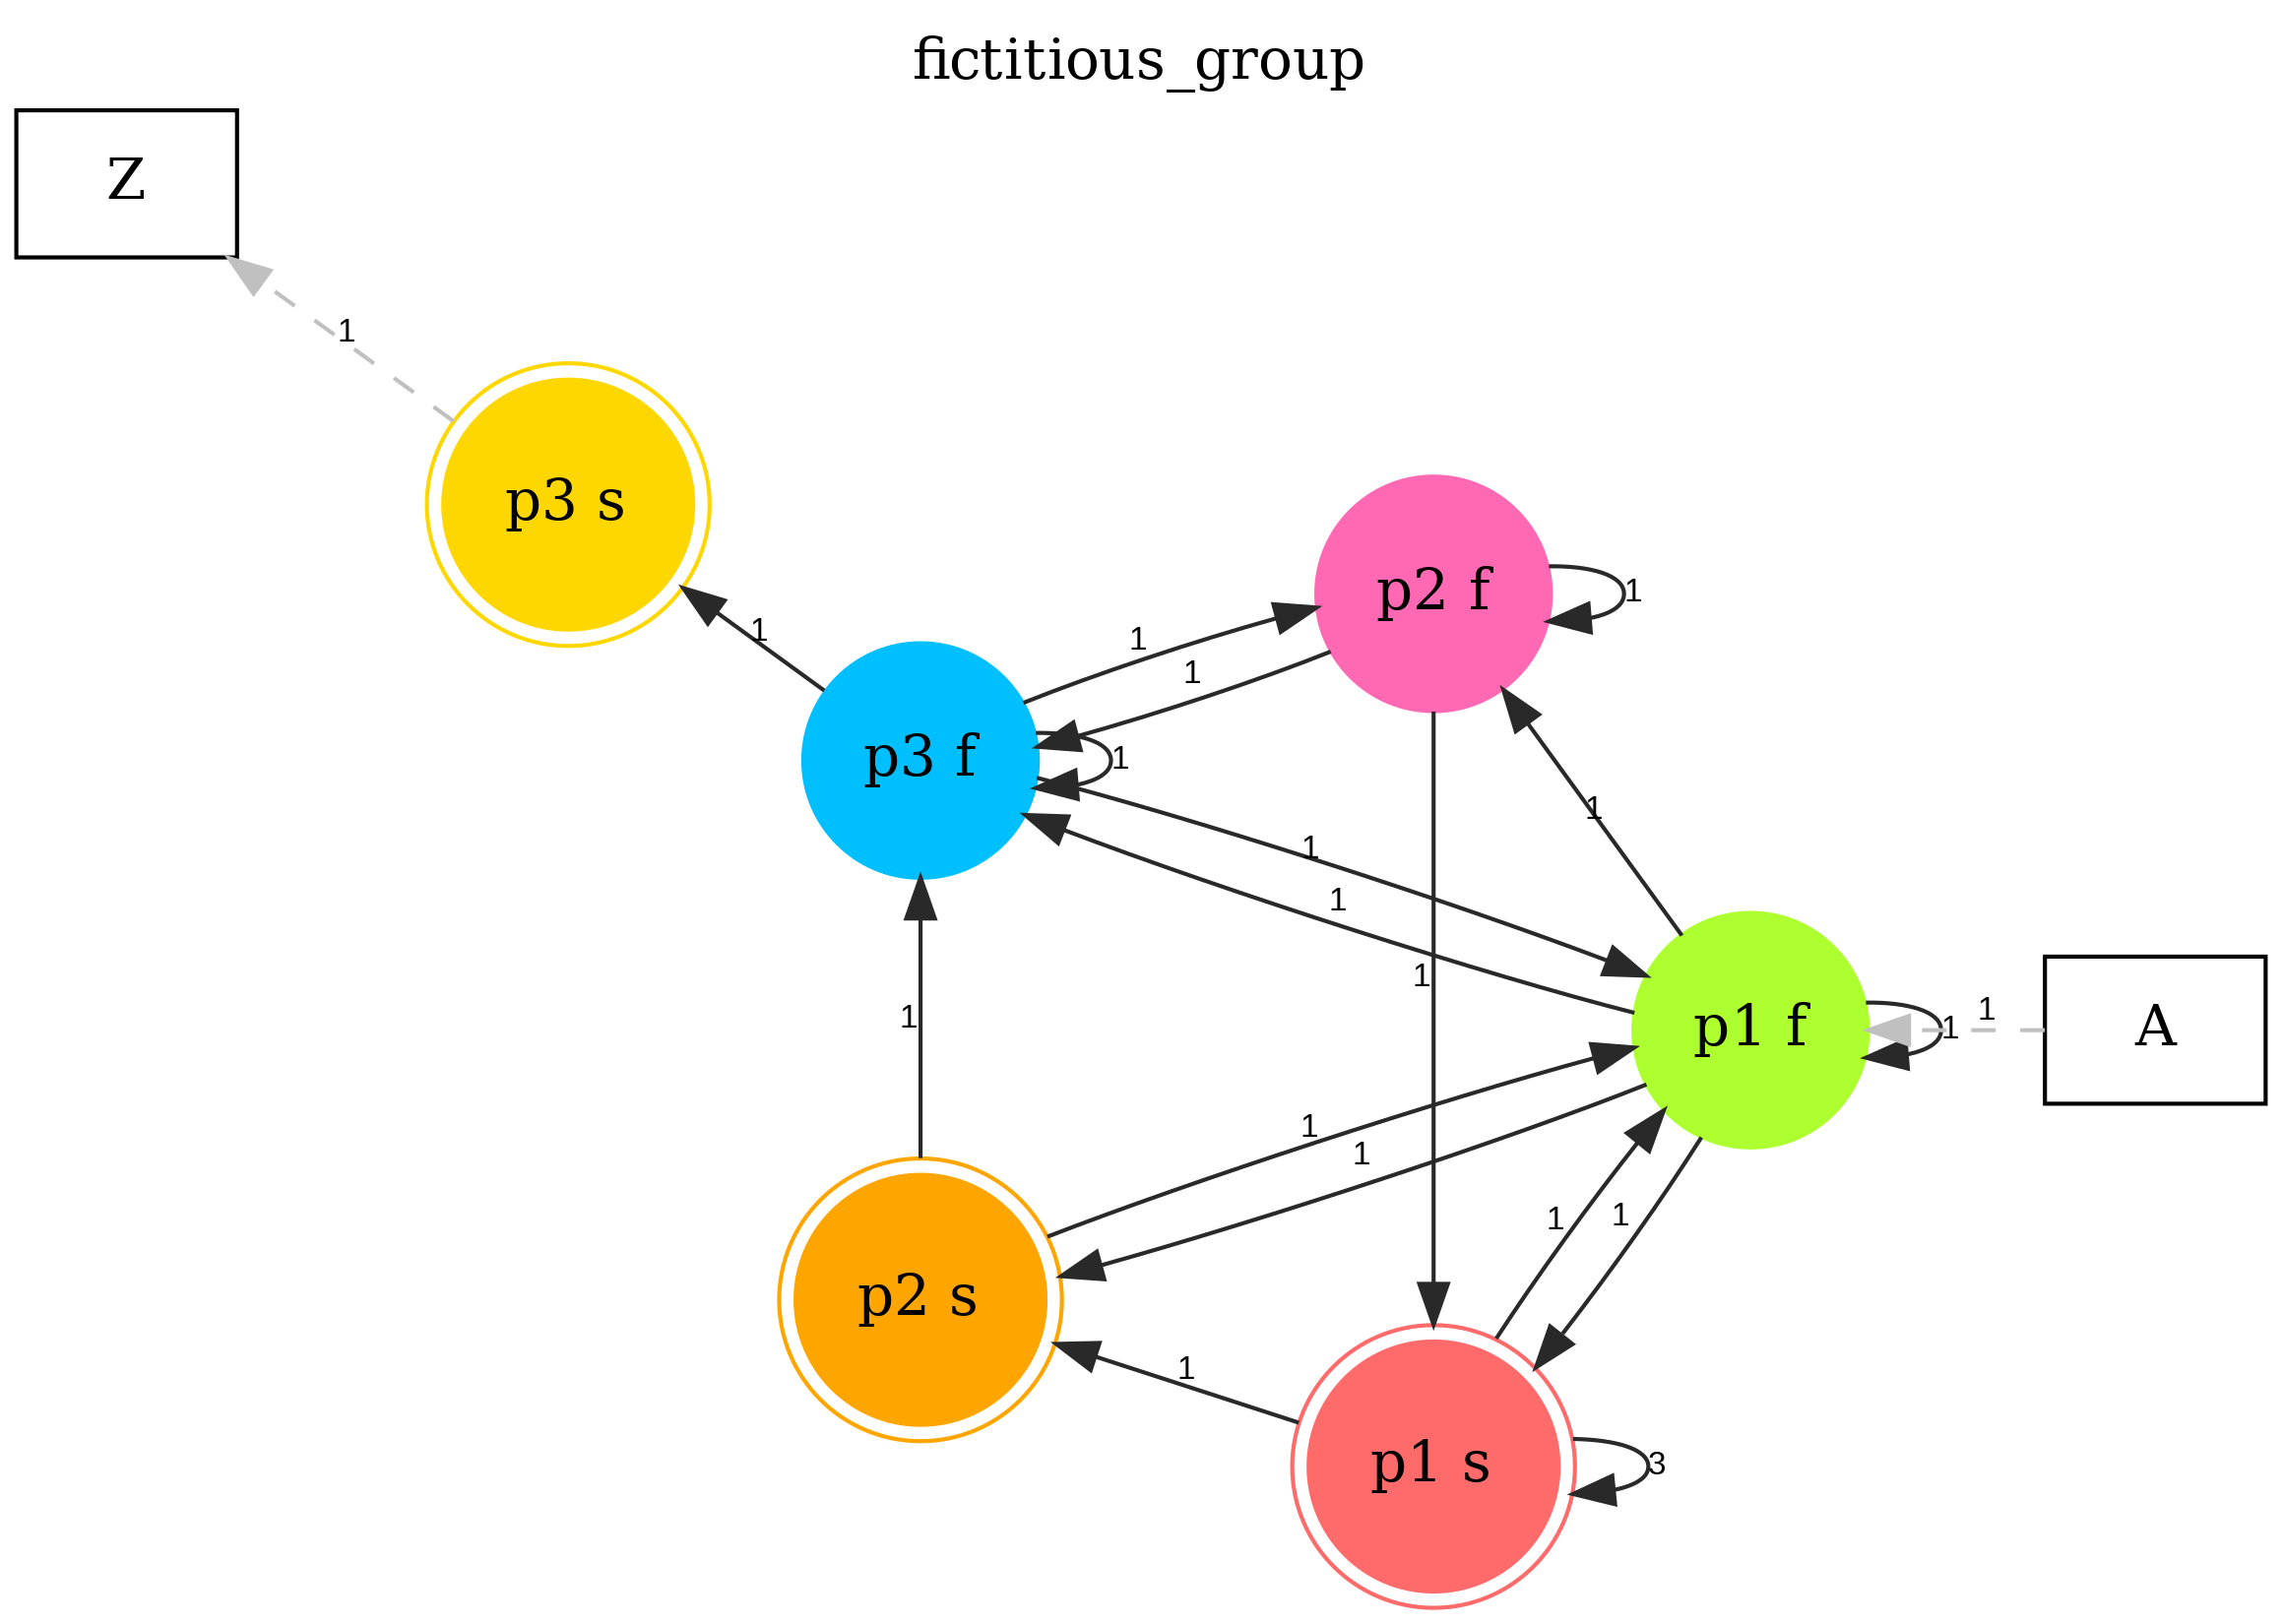
\includegraphics[width=0.47\textwidth]{implementación/examplecycles.png}}\qquad
\subfloat[El mismo grafo que el de la Figura \ref{fig:examplecycles} pero eliminando los ciclos
y manteniendo el grado de entrada de cada uno de los vértices.]{\label{fig:examplewithoutcycles}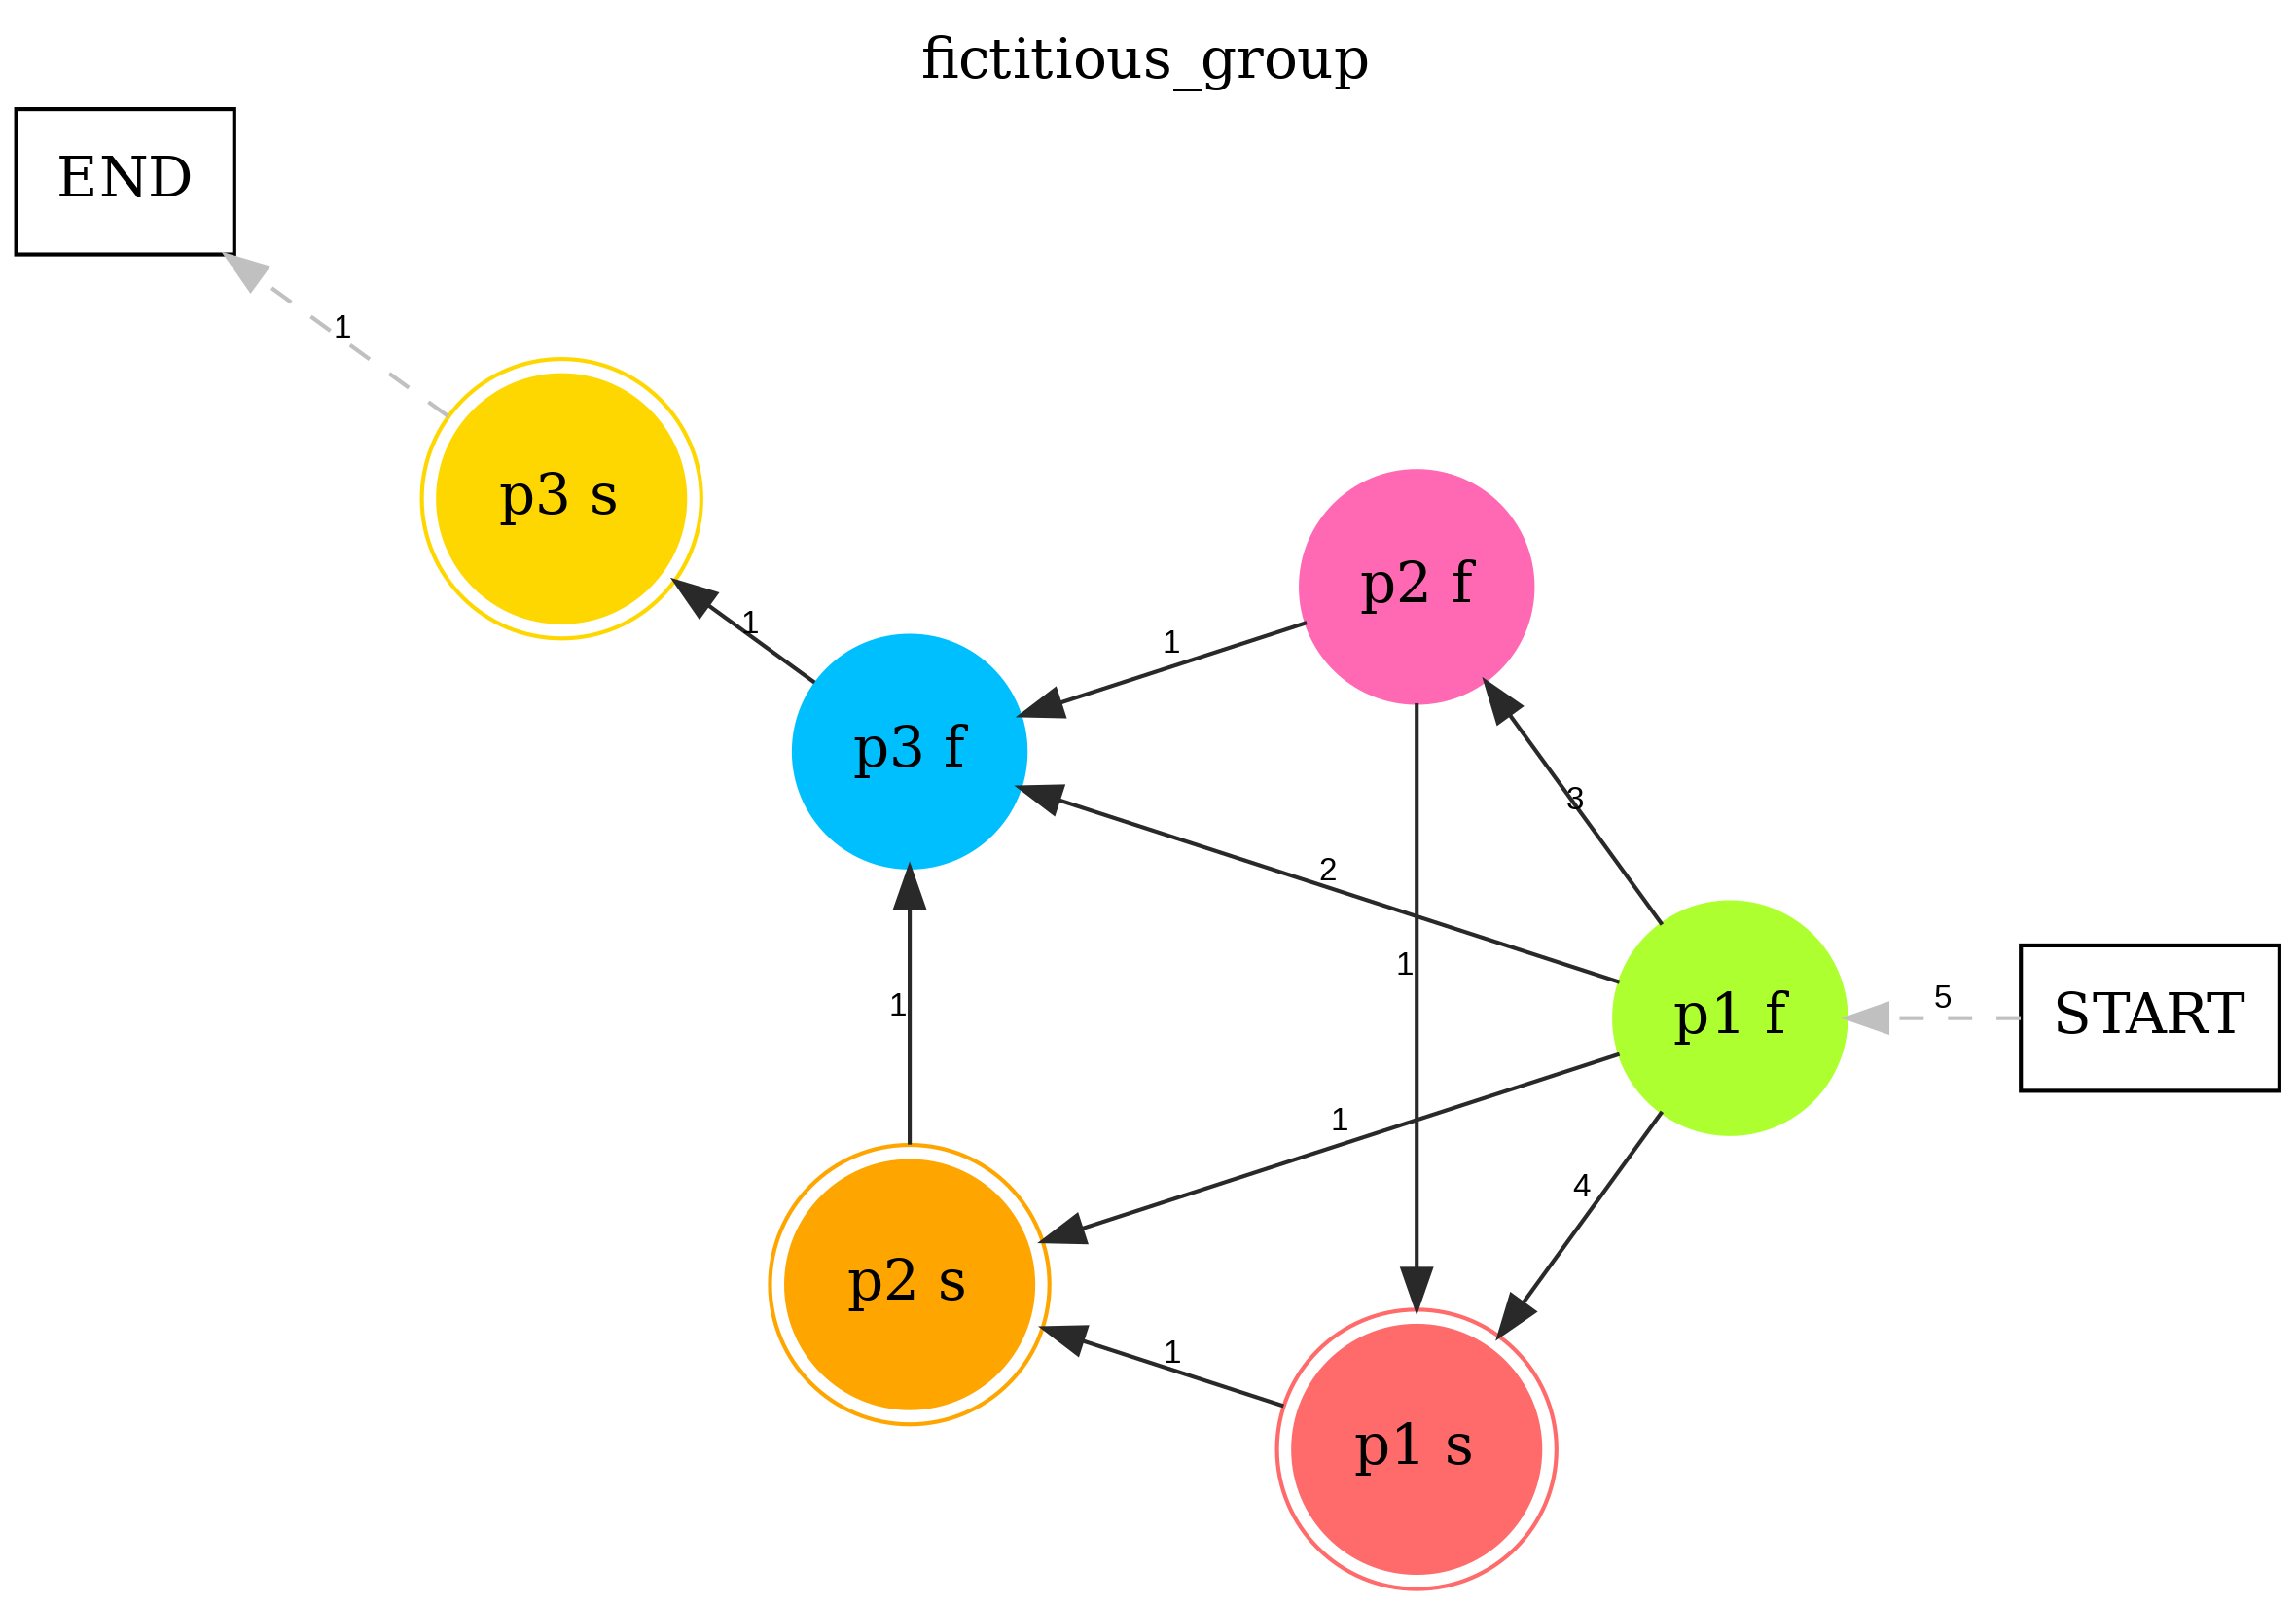
\includegraphics[width=0.47\textwidth]{implementación/examplewithoutcycles.png}}
\caption{Grafos resultantes de la continuación del ejemplo de la Sección \ref{sec:initial}.}
\label{fig:examples}
\end{figure}

\begin{equation}\label{eq:matrix}
\mathcal{A}^g = 
\left(
\begin{array}{c|cccccccc}
    & A & p_1^f & p_1^s & p_2^f & p_2^s & p_3^f & p_3^s & Z \\
  \hline
  A & \textbf{0} & 5 & 0 & 0 & 0 & 0 & 0 & 0 \\
  p_1^f & 0 & \textbf{0} & 4 & 3 & 1 & 2 & 0 & 0 \\
  p_1^s & 0 & 0 & \textbf{0} & 0 & 1 & 0 & 0 & 0 \\
  p_2^f & 0 & 0 & 1 & \textbf{0} & 0 & 1 & 0 & 0 \\
  p_2^s & 0 & 0 & 0 & 0 & \textbf{0} & 1 & 0 & 0 \\
  p_3^f & 0 & 0 & 0 & 0 & 0 & \textbf{0} & 1 & 0\\
  p_3^s & 0 & 0 & 0 & 0 & 0 & 0 & \textbf{0} & 1 \\
  Z & 0 & 0 & 0 & 0 & 0 & 0 & 0 & \textbf{0}
\end{array}
\right)
\end{equation}

Esta perspectiva nos permite ver $B^g$ como un grafo dirigido $G = (V^g,E^g)$ que capta la dinámica de un grupo mientras se esfuerza por resolver los distintos problemas que se le han planteado. Por lo tanto, el conjunto de eventos (problemas y estado de los mismos más un evento de inicio y otro de finalización) que los estudiantes han realizado es el conjunto de vértices del grafo:

\begin{equation}
V^g = \left\lbrace ^0A \right\rbrace \cup \left\lbrace ^sp_i^k \in B^g \right\rbrace \cup \left\lbrace Z \right\rbrace
\end{equation}

y cada par de eventos consecutivos se considera una arista del grafo:

\begin{equation}
E^g = \left\lbrace <x,y>, x = {}^sp_i^r, y = {}^tp_j^l, t = s+1, x,y \in B^g\right\rbrace
\end{equation}

que, de hecho, puede representarse como su matriz de adyacencia ponderada y nos permite representar el invariante grado de entrada.

\section{La matriz característica de un grupo}

Este grafo sigue siendo un grafo cíclico (Definición \ref{def:cyclic}) y, como estamos interesados en la representación más esencial del comportamiento de los estudiantes, se eliminarán esos ciclos quitando una cantidad mínima de aristas y conservando invariante el grado de entrada, obteniendo el grafo esencial de la Figura \ref{fig:examplewithoutcycles}, con su respectiva matriz de distancias (Ecuación \ref{eq:matrix}), que denominamos matriz característica (Definición \ref{def:adjacency}) del grupo $g$, $\mathcal{A}^g$. Esta matriz característica es una representación minimal de $B^g$ y a partir de ella se pueden extraer numerosas métricas, siendo la más importante una medida de la complejidad inherente a $B^g$.

Por lo tanto, $\mathcal{A}^g[x,y] = d > 0$ significaría que $x$ precede a $y$ $d$ veces en $B^g$. Así pues, cuanto mayor sea $d$, mayor será la influencia de $x$ sobre $y$ en términos del comportamiento codificado en $\mathcal{A}^g$. En aras de la simplicidad, además del uso de valores enteros para obtener una fila o columna, también se utilizarán los nombres identificativos de los nodos como, por ejemplo, se muestra en la Ecuación \ref{eq:example}.

\begin{equation}\label{eq:example}
\mathcal{A}[1,2] = \mathcal{A}[p_2^f,p_3^f] = 4
\end{equation}

Podría decirse que $\mathcal{A}^g$ contiene lo que podría haber sido la \emph{experiencia} de resolver todos los problemas, es decir, una especie de huella que codifica la relación entre fracaso y éxito y la fuerza de estas relaciones. Vale la pena decir que en todos los registros (Tabla \ref{tab:records}) todas estas matrices son diferentes entre sí. Se derivarán otras dos matrices de $\mathcal{A}^g$. En primer lugar, obtendremos una matriz de adyacencia característica integrada únicamente por ceros y unos a la que denotaremos $\mathcal{A}'$. Así pues, $\mathcal{A}'[r, c]$ será $1$ únicamente cuando $\mathcal{A}[r, c] > 0$. En segundo lugar, calcularemos la matriz de distancias mínimas que se obtendrá mediante la aplicación del algoritmo de caminos mínimos de Dijkstra, de modo que $\hat{\mathcal{A}}[r, c]$ contiene una especie de longitud de camino mínima entre los diferentes nodos del grafo en función del número de sesiones. Por tanto, estas estructuras son un punto de partida ideal desde el que decodificar la información sobre las experiencias de aprendizaje. En particular, nuestro principal interés será determinar si existe una relación entre esta estructura y el éxito o el fracaso de cada uno de los grupos de alumnos. Es decir, ¿un mal comportamiento de los alumnos produciría un grafo mal estructurado? Y viceversa, ¿las medidas estándar de calidad y entropía definidas puramente sobre grafos permiten detectar grupos en riesgo? La respuesta, resulta ser sí (Capítulo \ref{sec:chapterXIII}).

\section{Resultados obtenidos}

En esta sección se muestran los diferentes grafos obtenidos con la herramienta de Minería de Procesos \emph{Graph Miner}. Comparando las Figuras \ref{fig:DBA1516P2GA1} y \ref{fig:problemsDBA1516P2GA} vemos que los diagramas de la implementación propia y el original obtenido con Disco coinciden, con la salvedad de que en el diagrama de creación propia se muestran el $100\%$ de las actividades y el $100\%$ de los caminos.

\begin{figure}[H]
    \centering
    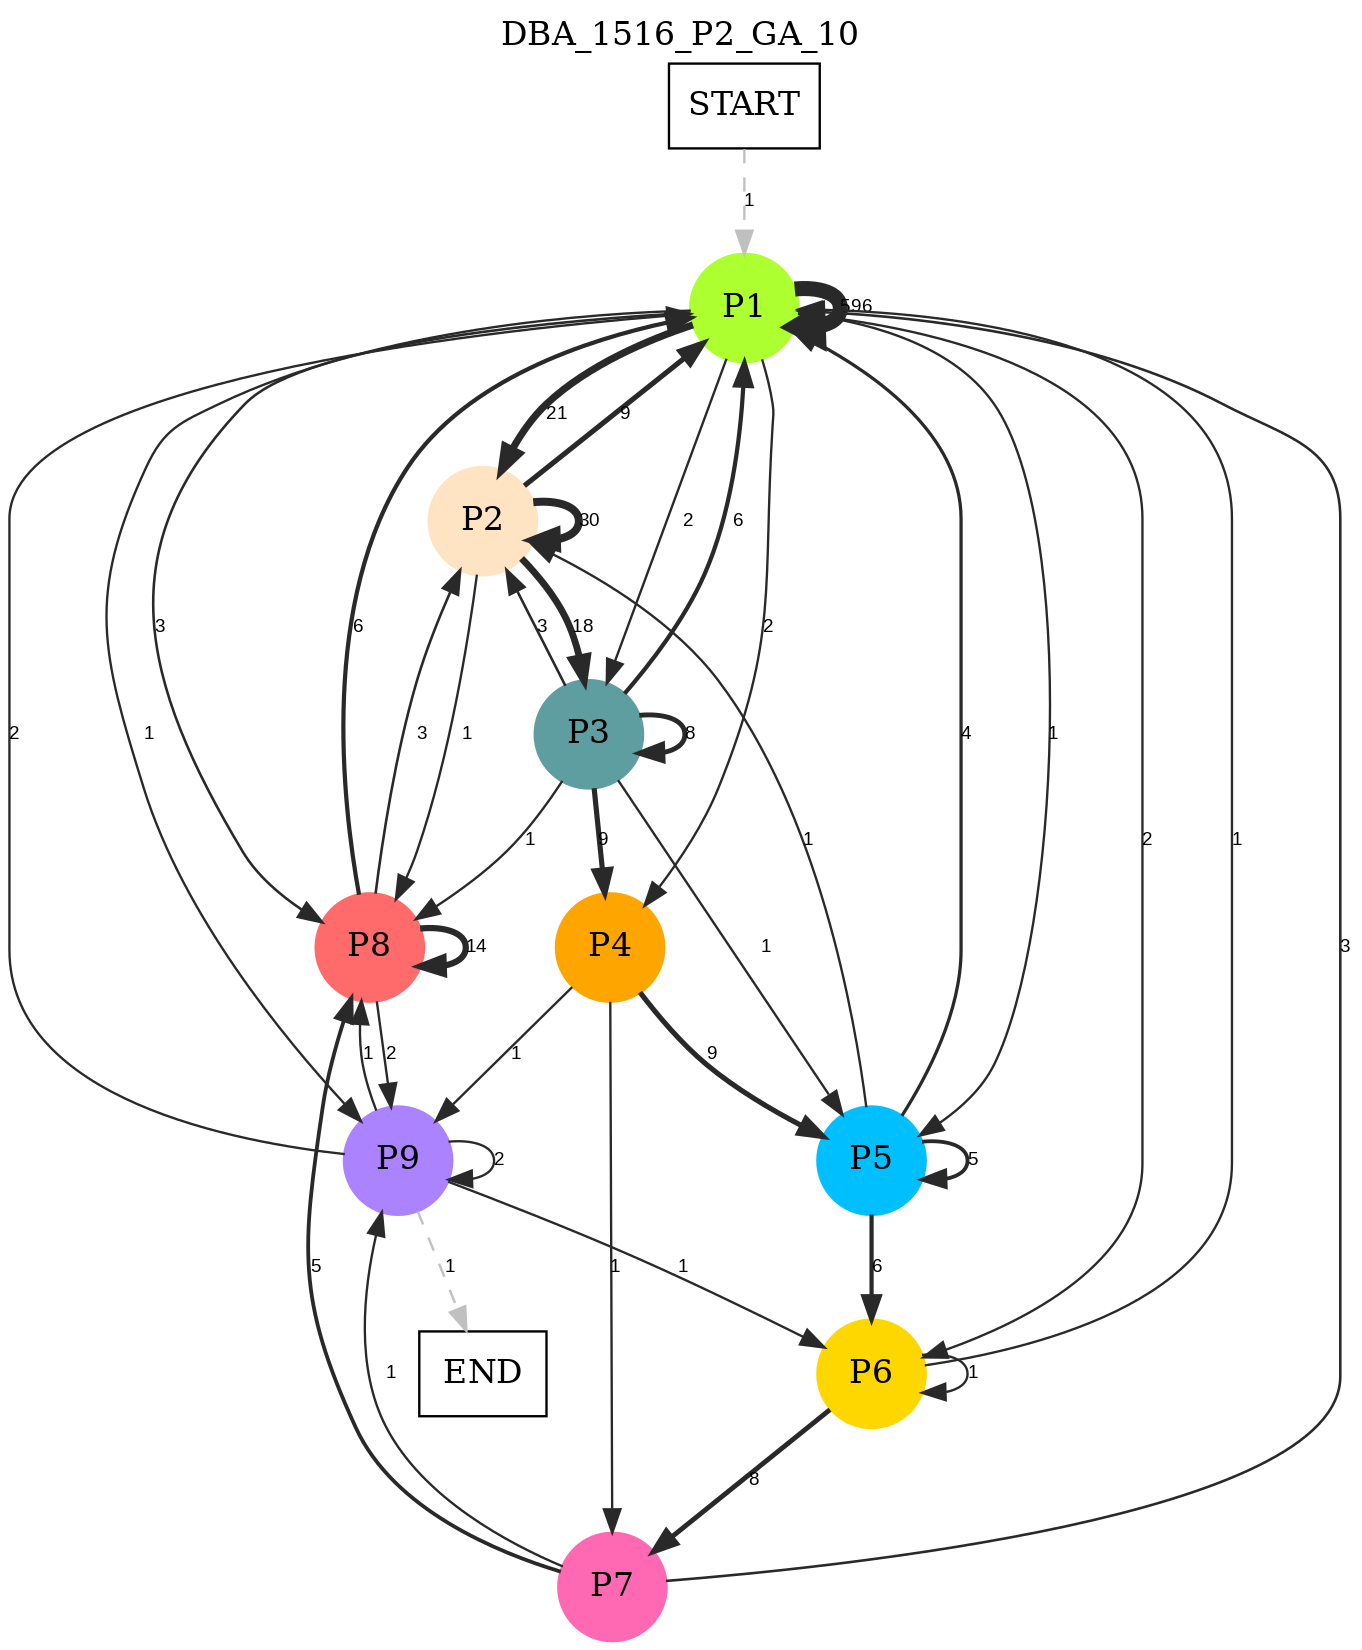
\includegraphics[width=0.5\textwidth]{implementación/DBA_1516_P2_GA_10_problems.png}
    \caption{Análisis de procesos del grupo \texttt{DBA 1516 P2 GA} (\texttt{Activity} problema y \texttt{CaseId} grupo) obtenido con la implementación propia.}
    \label{fig:DBA1516P2GA1}
\end{figure}

Además, como podemos ver en la Figura \ref{fig:DBA1516P2GA2}, hemos obtenido el mismo diagrama que el que se muestra en la Figura \ref{fig:compoundDBA1516P2GA} con la salvedad de que hemos impedido el retorno a un estado anterior (es decir, se han eliminado ciclos) y como, en el caso anterior, de que en el diagrama de creación propia se muestran el $100\%$ de las actividades y el $100\%$ de los caminos.

\begin{figure}[H]
    \centering
    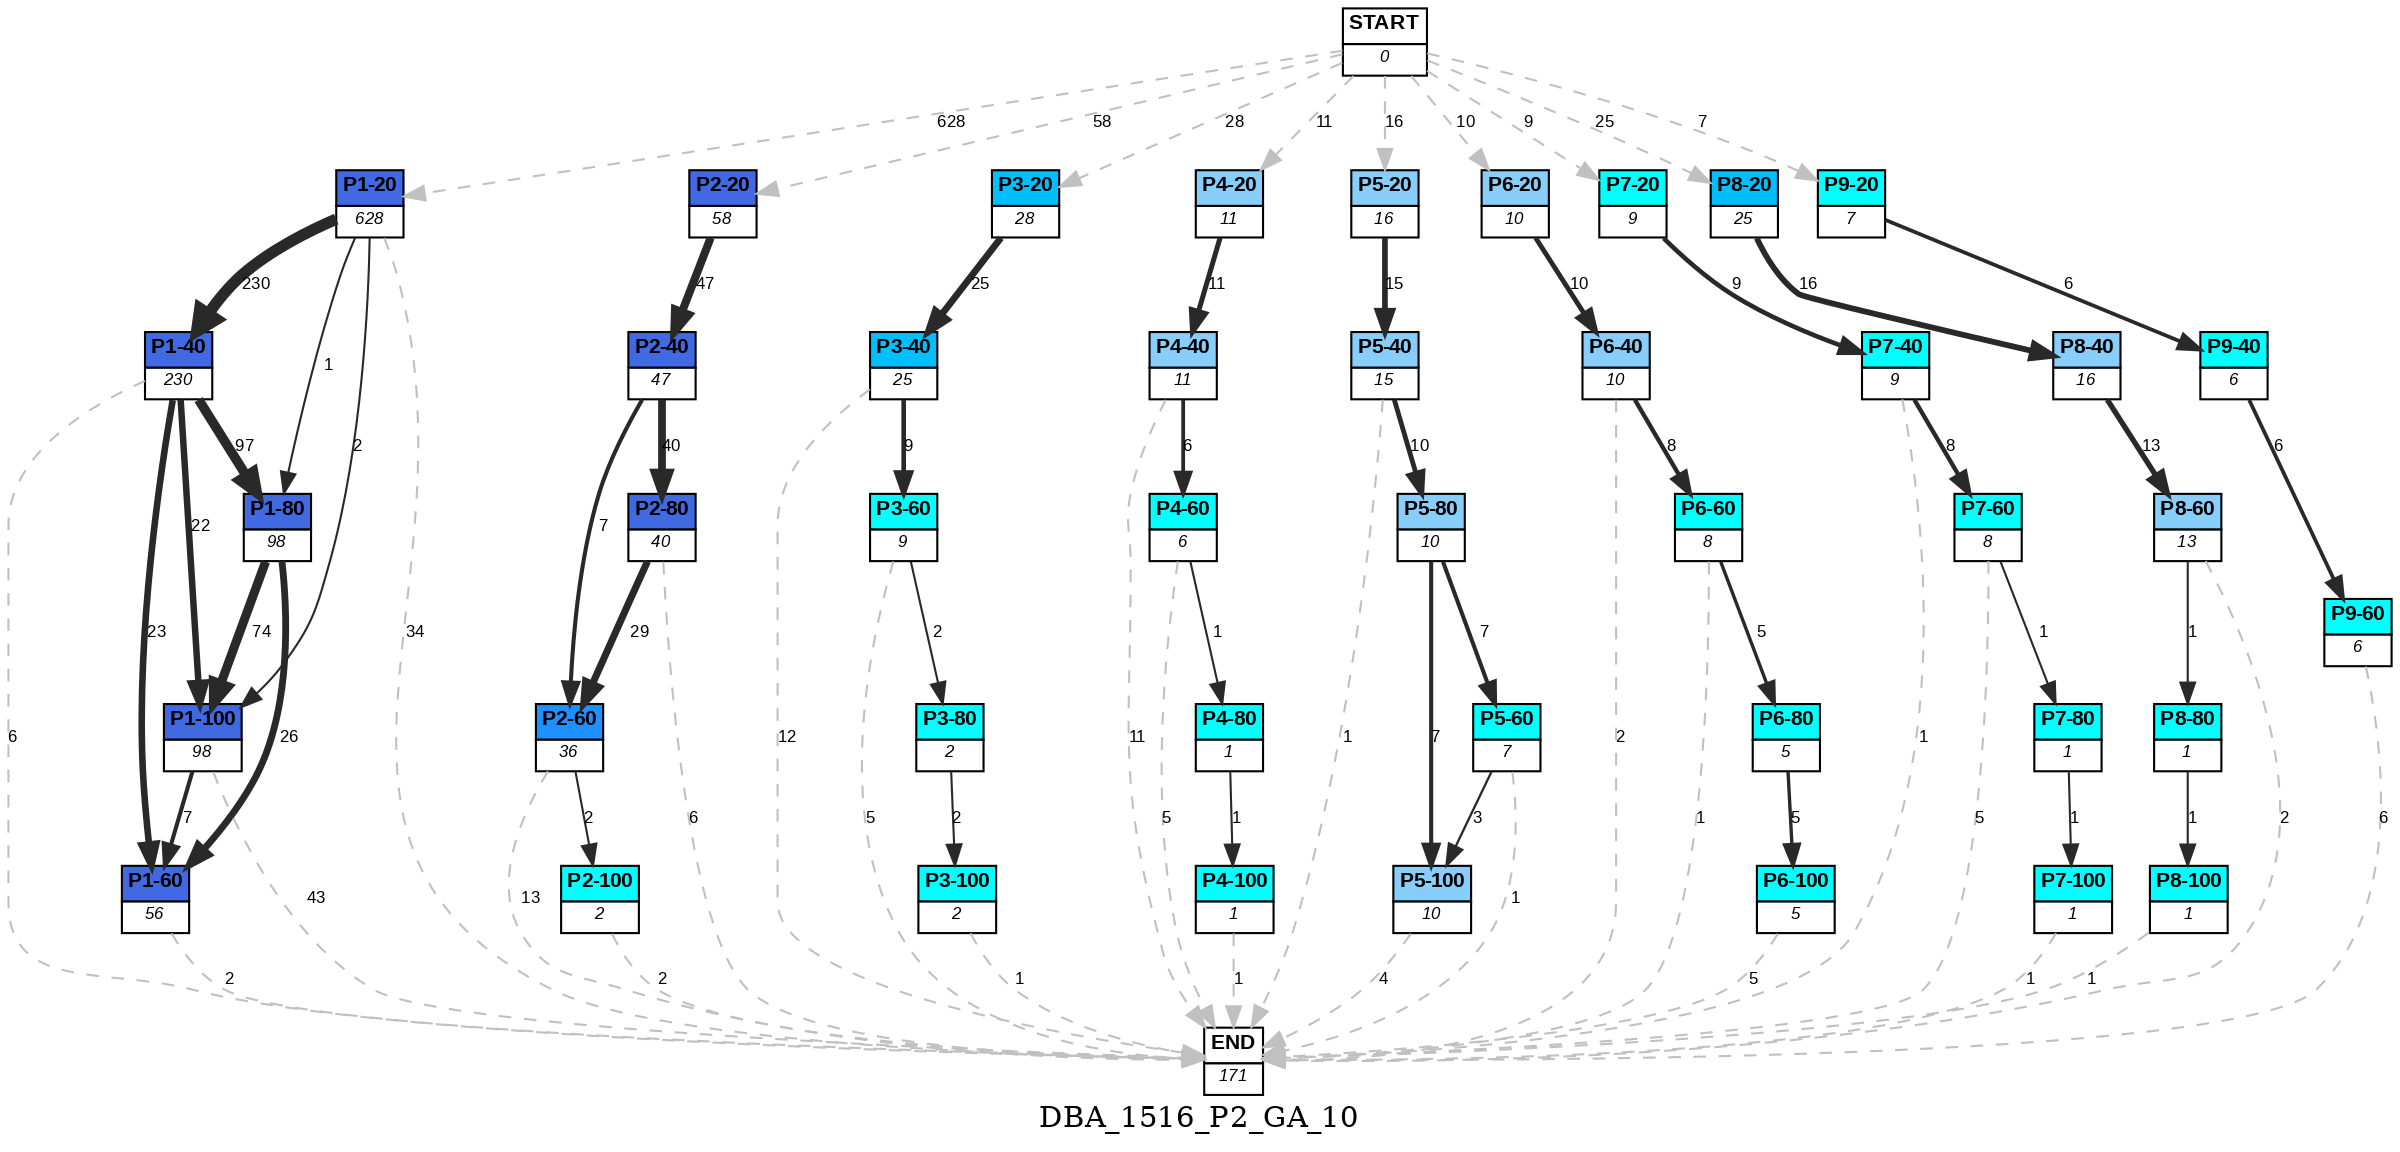
\includegraphics[width=\textwidth]{implementación/DBA_1516_P2_GA_10.png}
    \caption{Análisis de procesos del grupo \texttt{DBA 1516 P2 GA} (\texttt{Activity} problema-milestone y \texttt{CaseId} sesión) obtenido con la implementación propia.}
    \label{fig:DBA1516P2GA2}
\end{figure}

Además, se ha extendido la implementación de la herramienta de minería de procesos Disco \cite{gunther2012disco}, obteniendo otros diagramas que nos serán de mucha utilidad, como la agrupación en estados exitosos y fallidos (Figura \ref{fig:DBA1516P2GA3}) y una serie de grafos parciales considerando sólo la resolución hasta el problema $i$-ésimo, $i \in \left\lbrace 1,\dots,9 \right\rbrace$ (Figuras \ref{fig:DBA1516P2GA4}, \ref{fig:DBA1516P2GA5}, \ref{fig:DBA1516P2GA6} y \ref{fig:DBA1516P2GA7}) y considerando todos los registros, incluida toda la actividad realizada por el alumnado después de la resolución del último de los problemas ($i = 10$).

\begin{figure}[H]
    \centering
    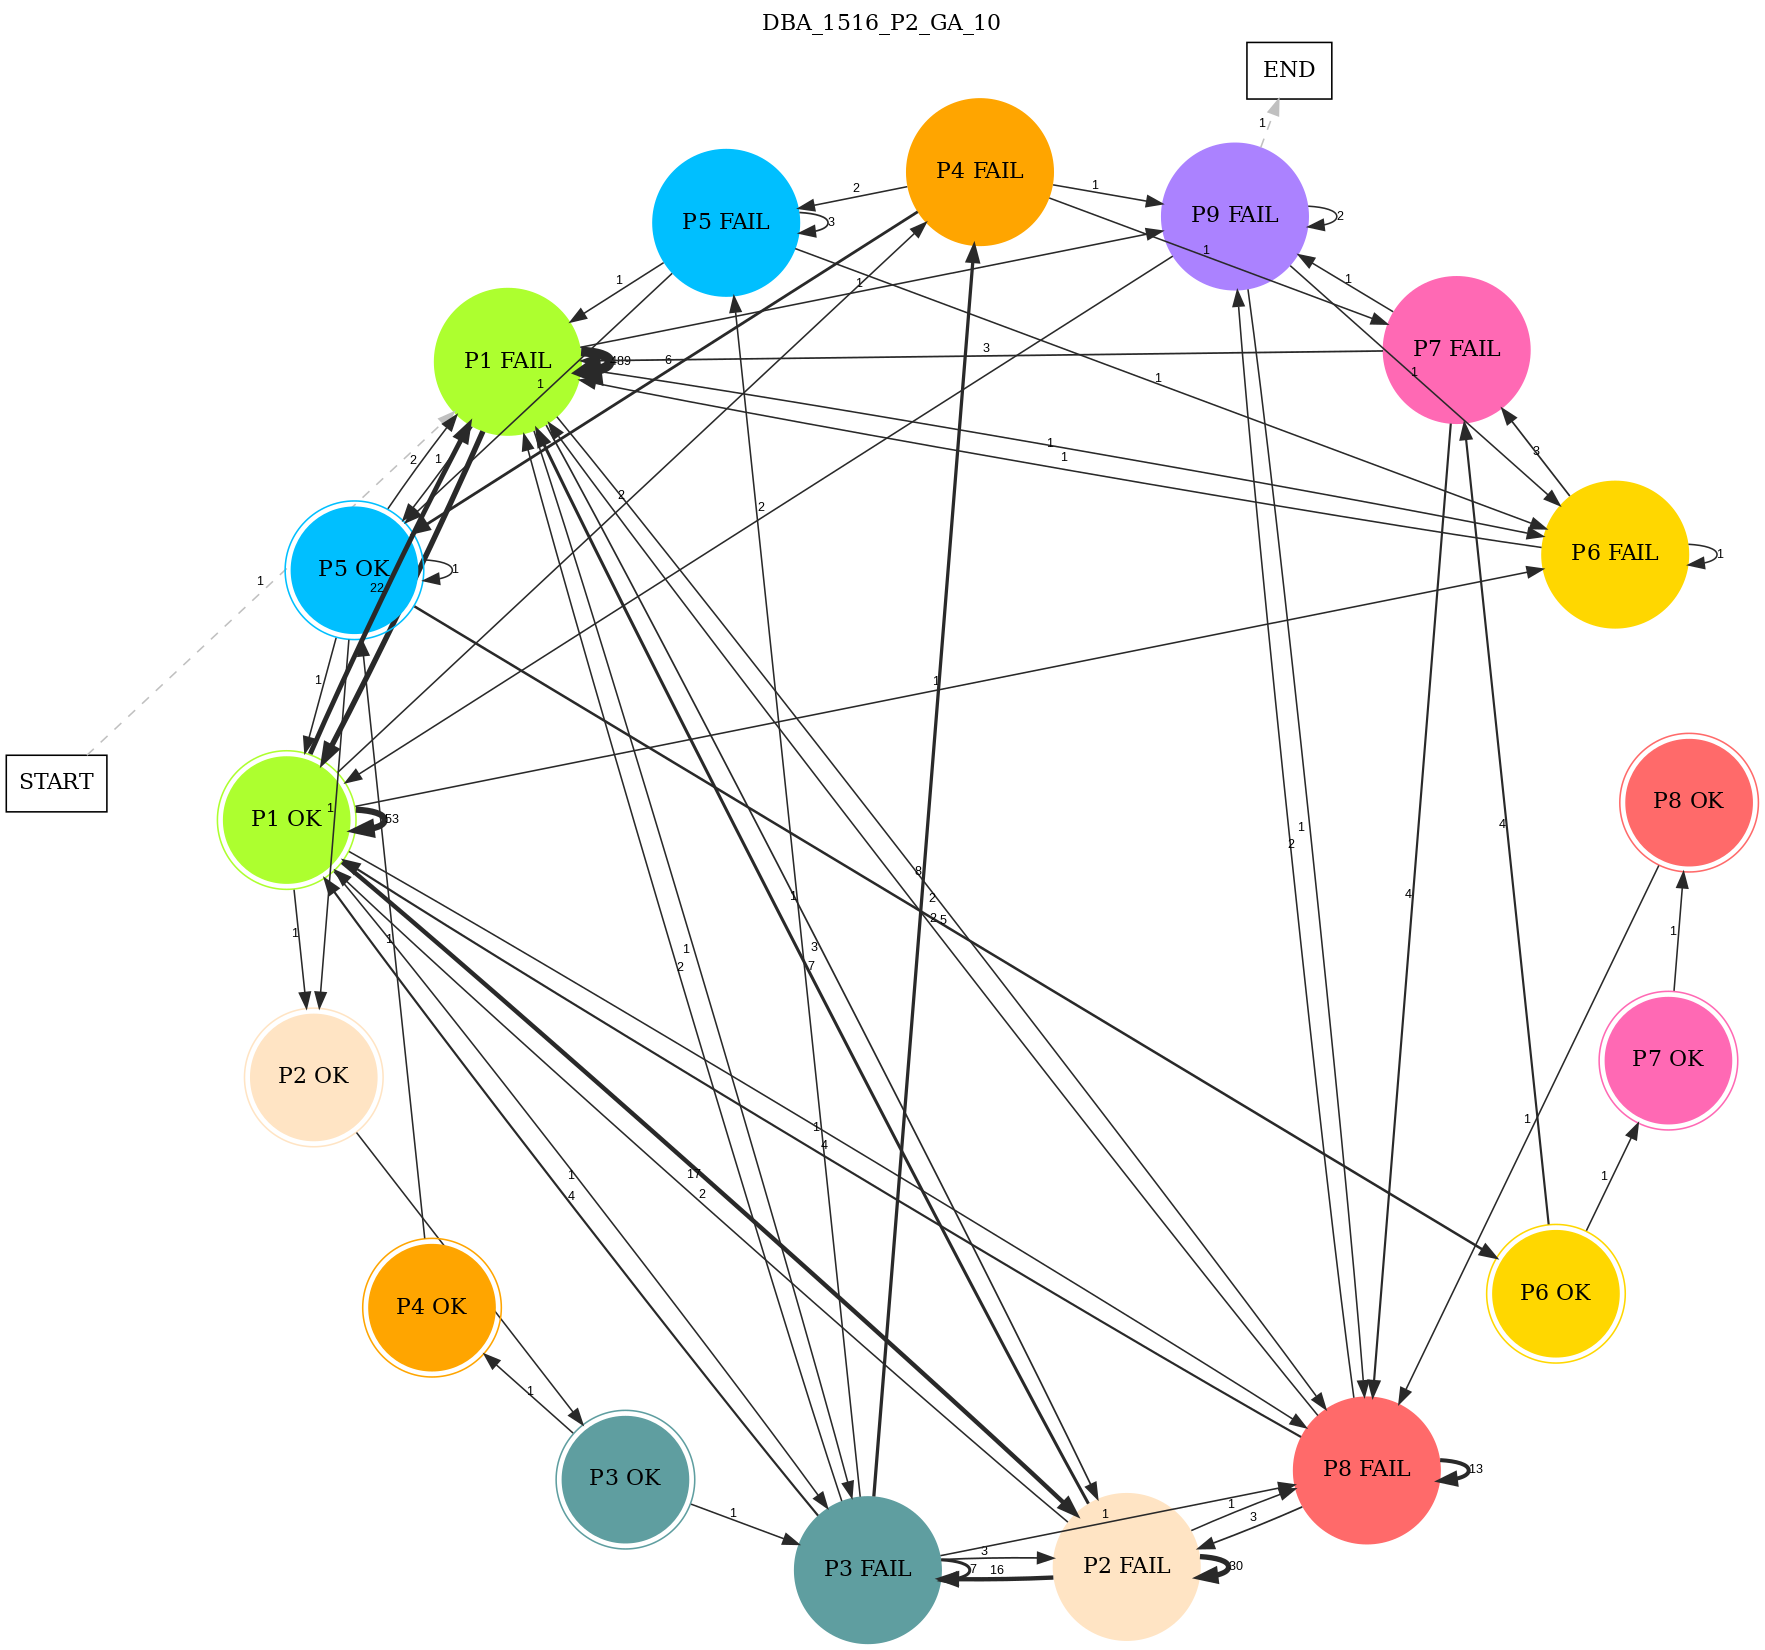
\includegraphics[width=0.7\textwidth]{implementación/DBA_1516_P2_GA_10_states.png}
    \caption{Análisis de procesos del grupo \texttt{DBA 1516 P2 GA} (\texttt{Activity} problema-estado y \texttt{CaseId} sesión) obtenido con la implementación propia.}
    \label{fig:DBA1516P2GA3}
\end{figure}

\begin{figure}[H]
\centering
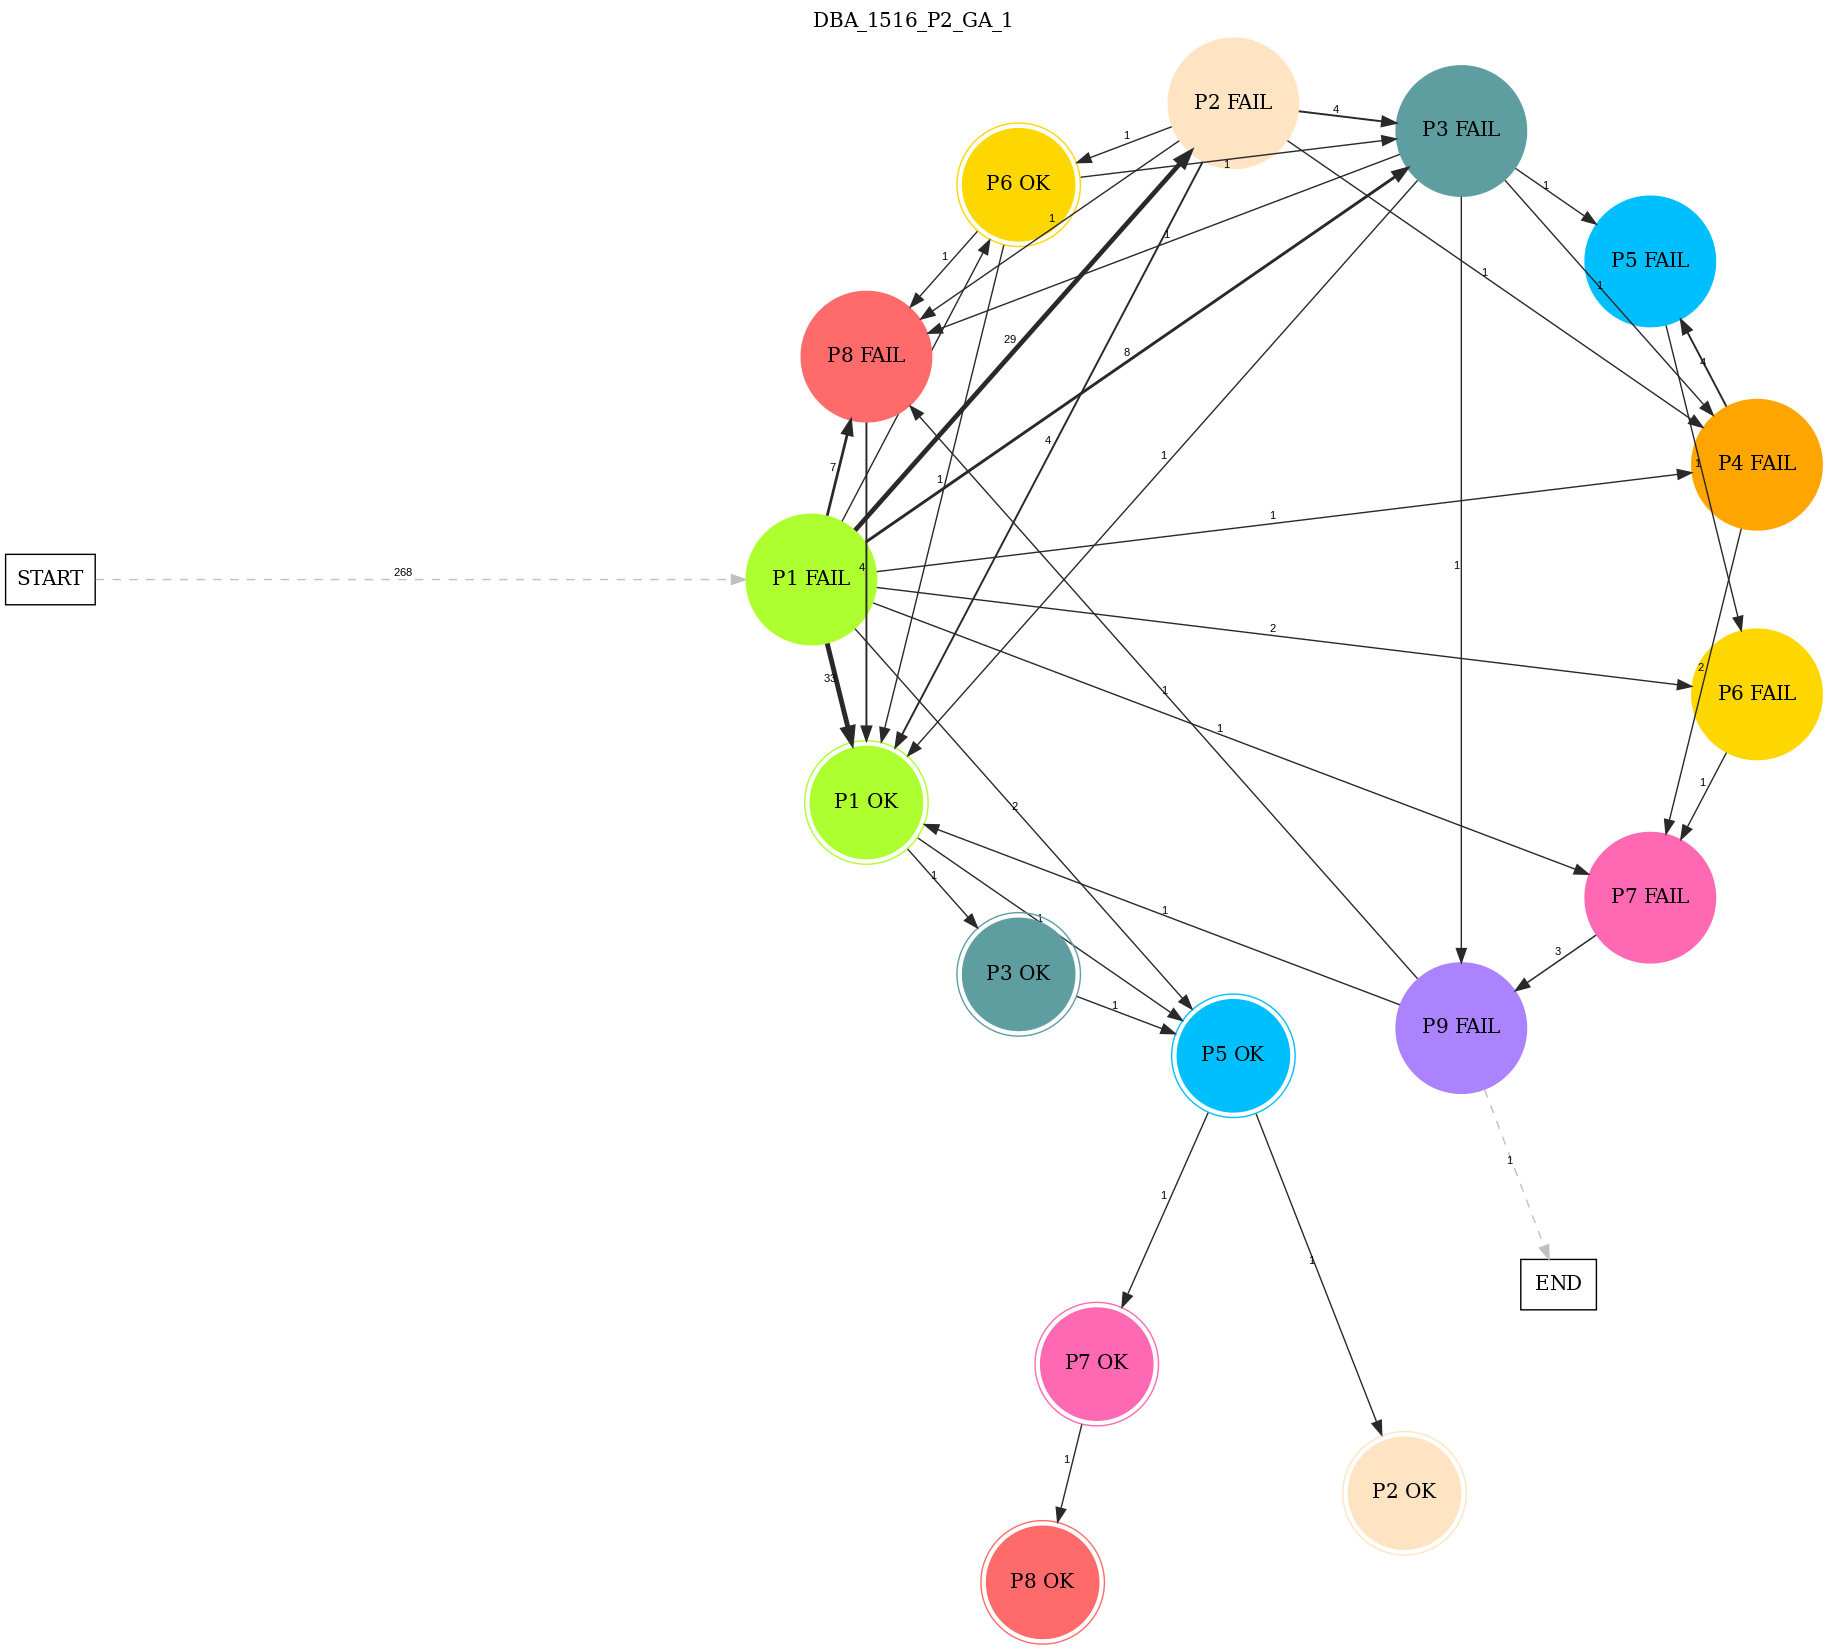
\includegraphics[width=0.5\textwidth]{implementación/DBA_1516_P2_GA_1.png} \\
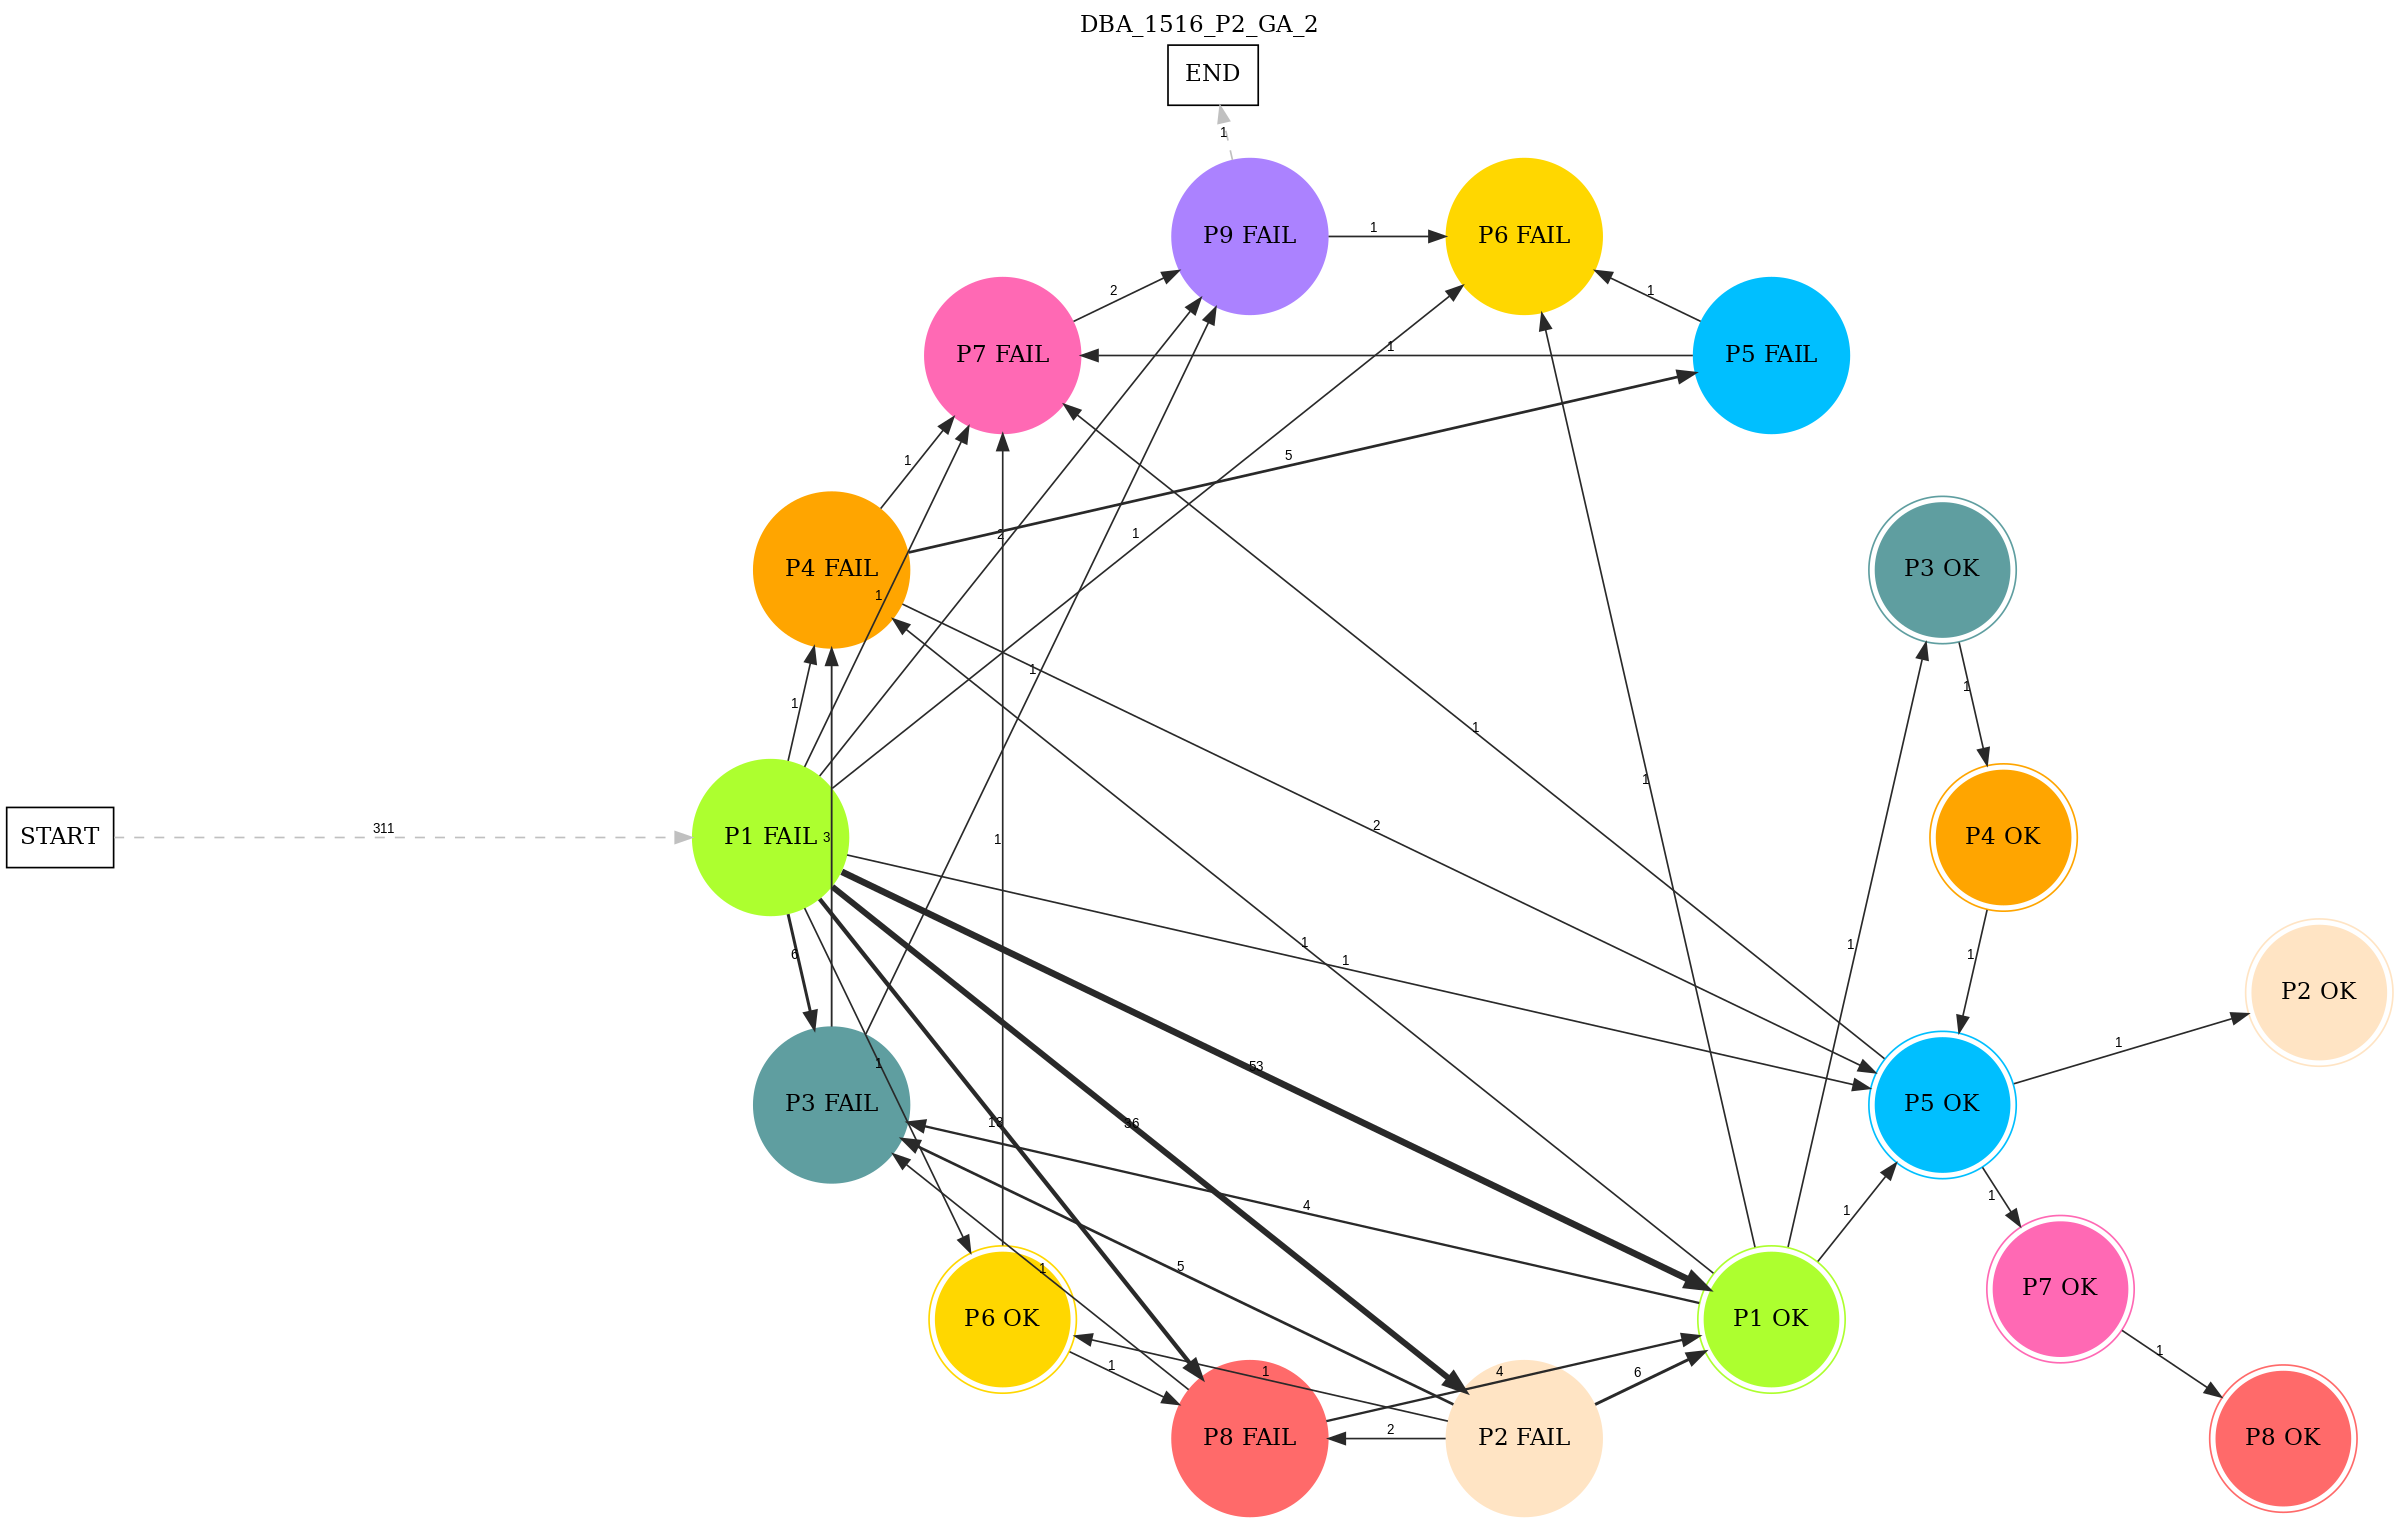
\includegraphics[width=\textwidth]{implementación/DBA_1516_P2_GA_2.png} \\
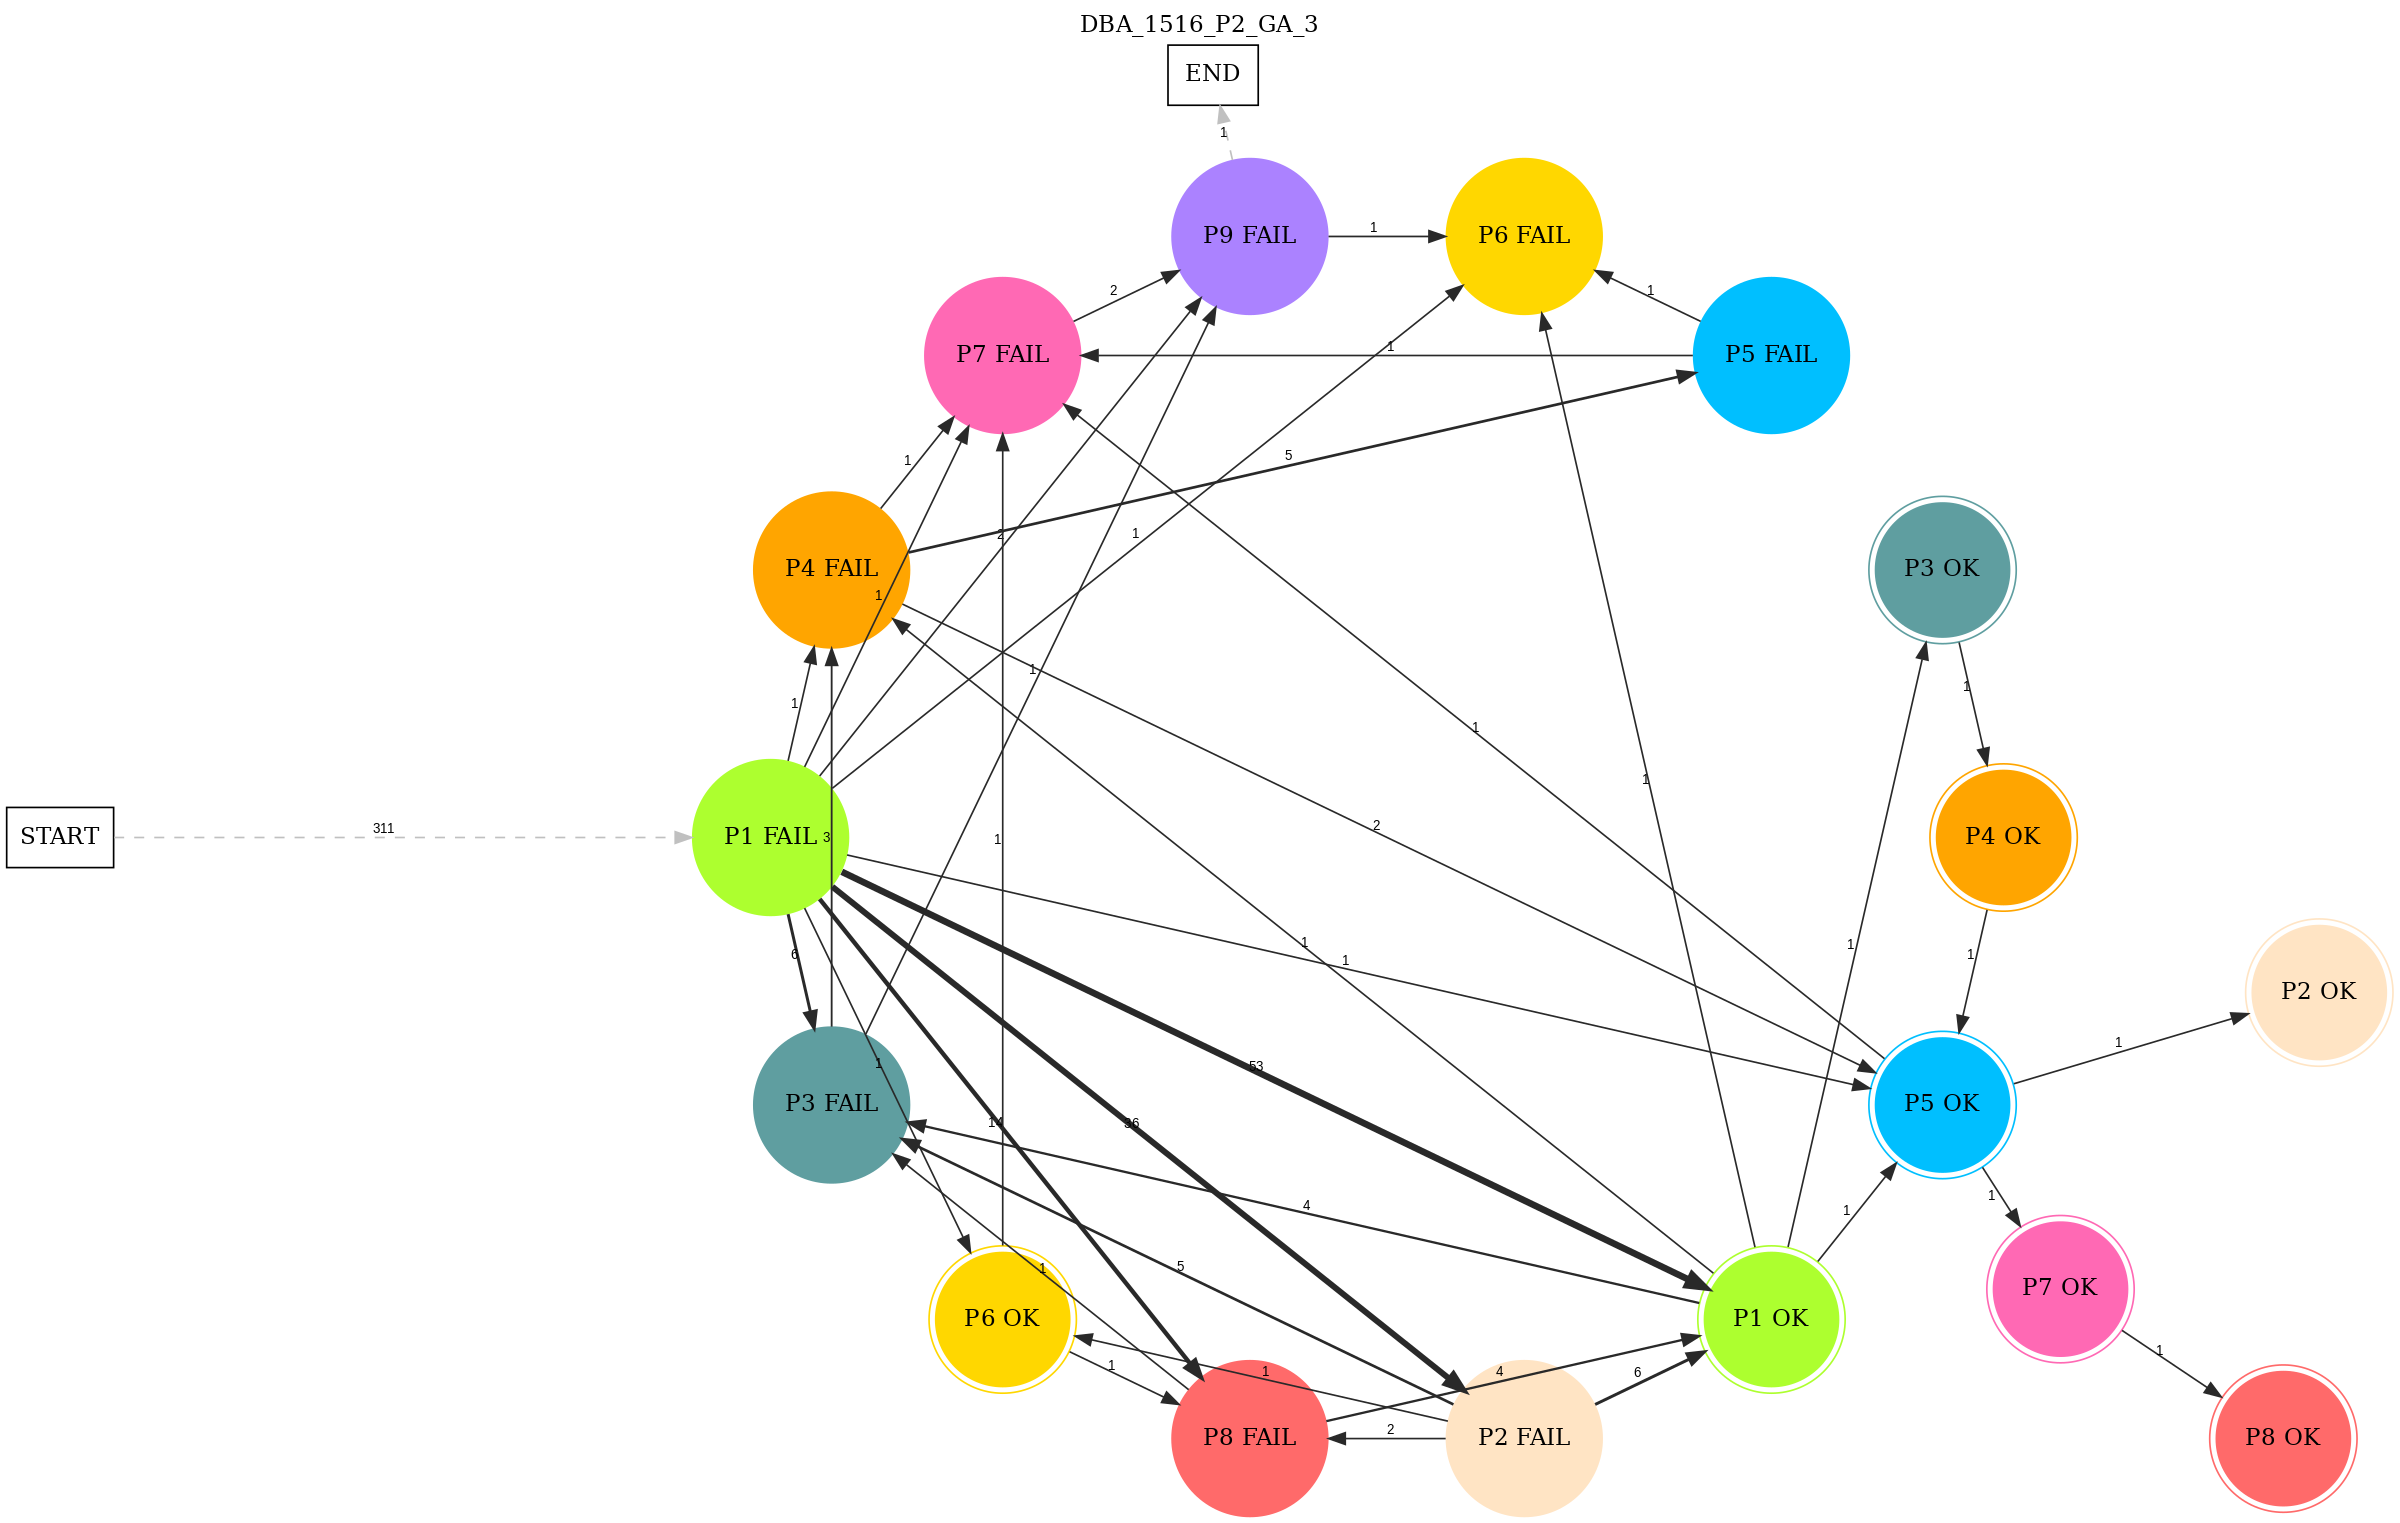
\includegraphics[width=\textwidth]{implementación/DBA_1516_P2_GA_3.png} \\
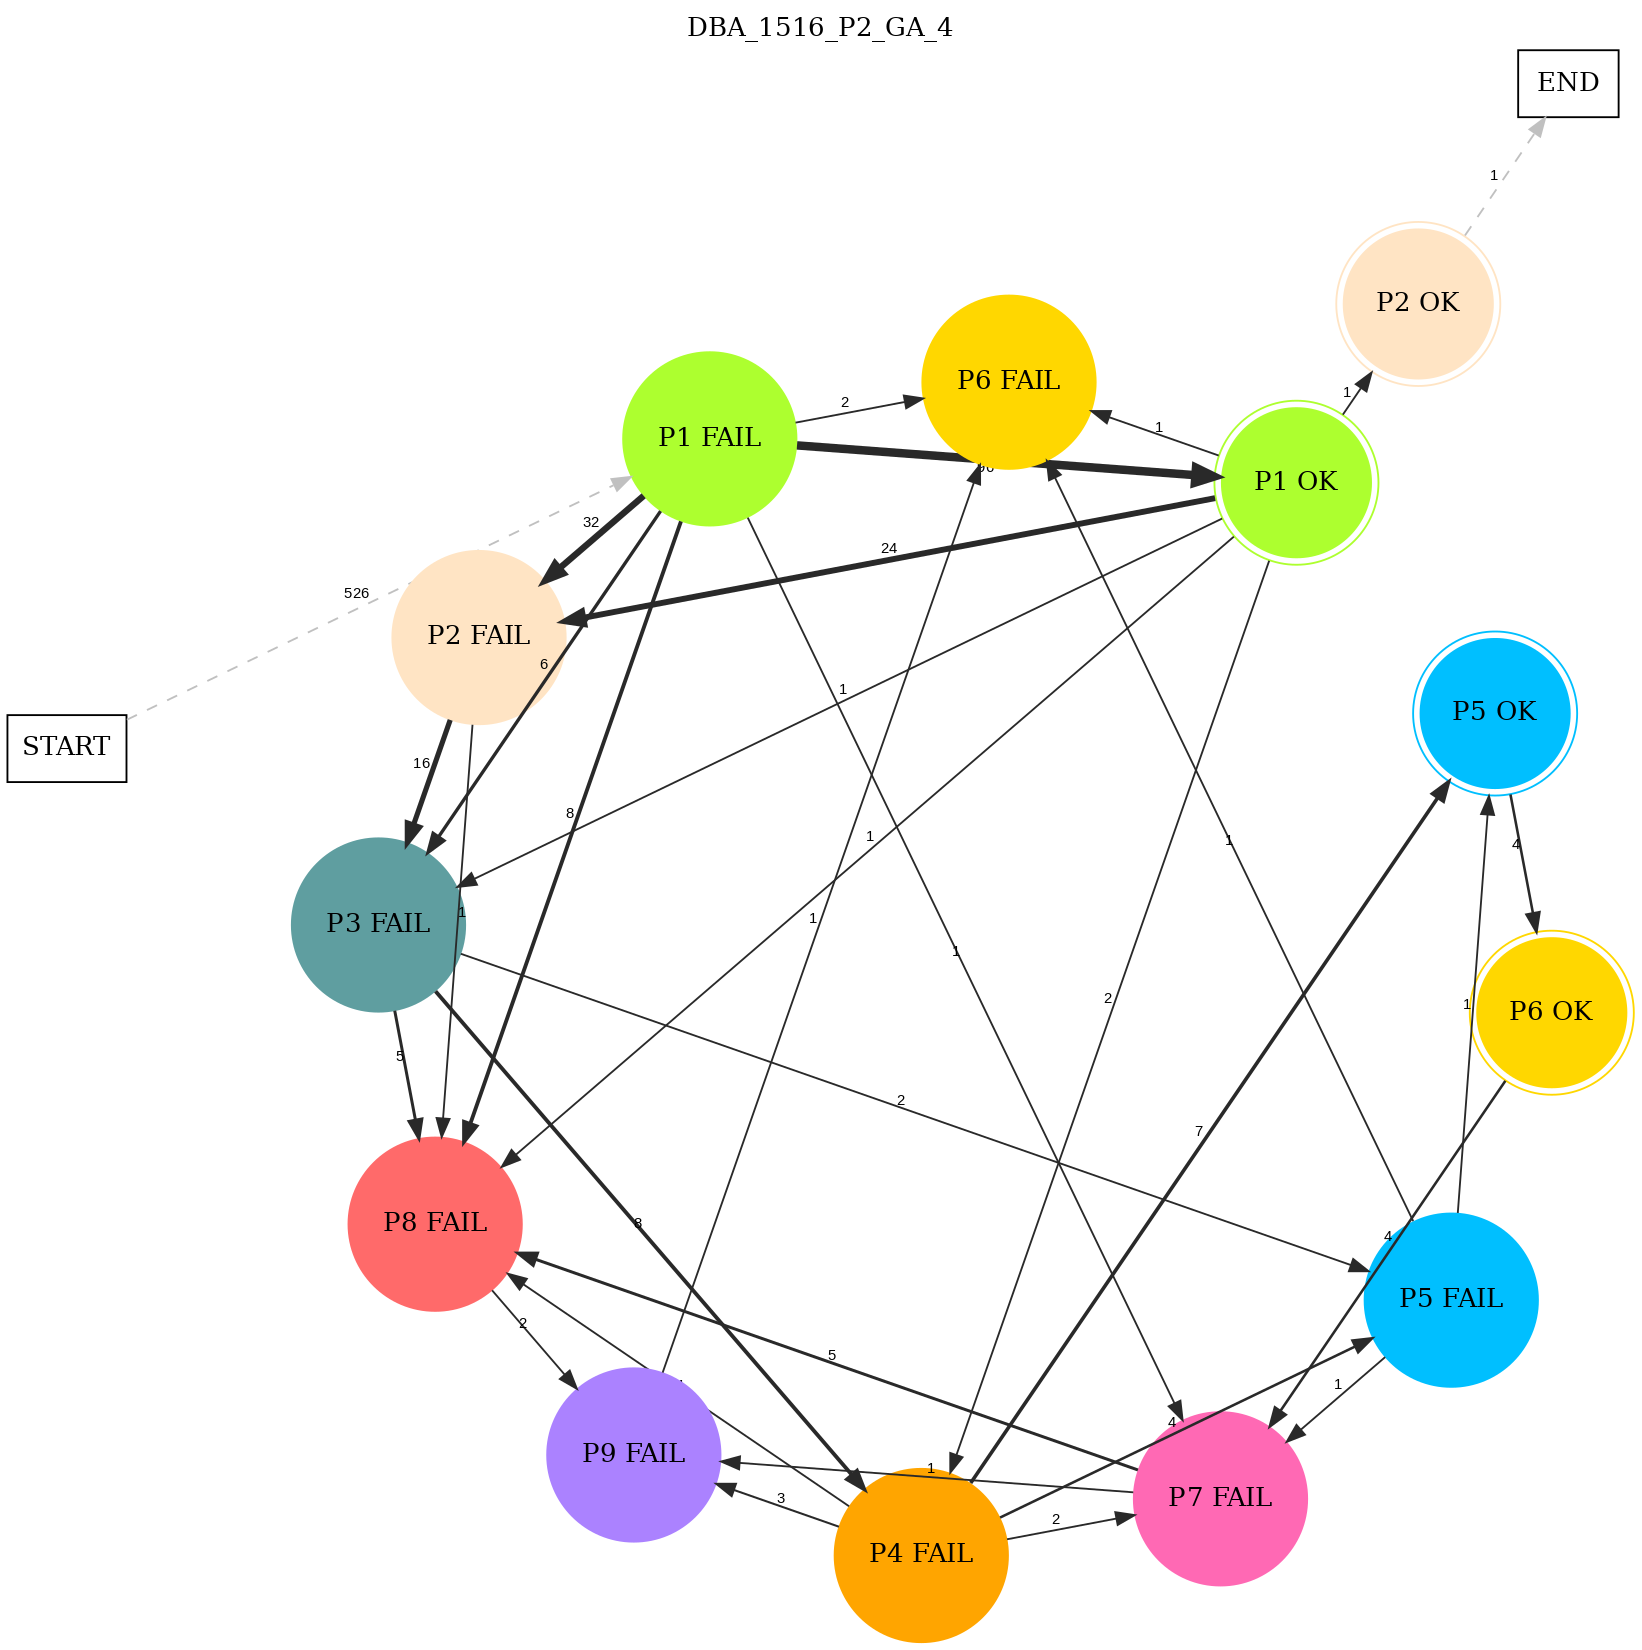
\includegraphics[width=0.7\textwidth]{implementación/DBA_1516_P2_GA_4.png}
\caption{Análisis de procesos del grupo \texttt{DBA 1516 P2 GA} (\texttt{Activity} problema-estado y \texttt{CaseId} sesión) obtenido con la implementación propia. En estos grafos los ciclos se han eliminado con el procedimiento explicado en la Sección \ref{sec:representation}.}
\label{fig:DBA1516P2GA4}
\end{figure}

\begin{figure}[H]
\centering
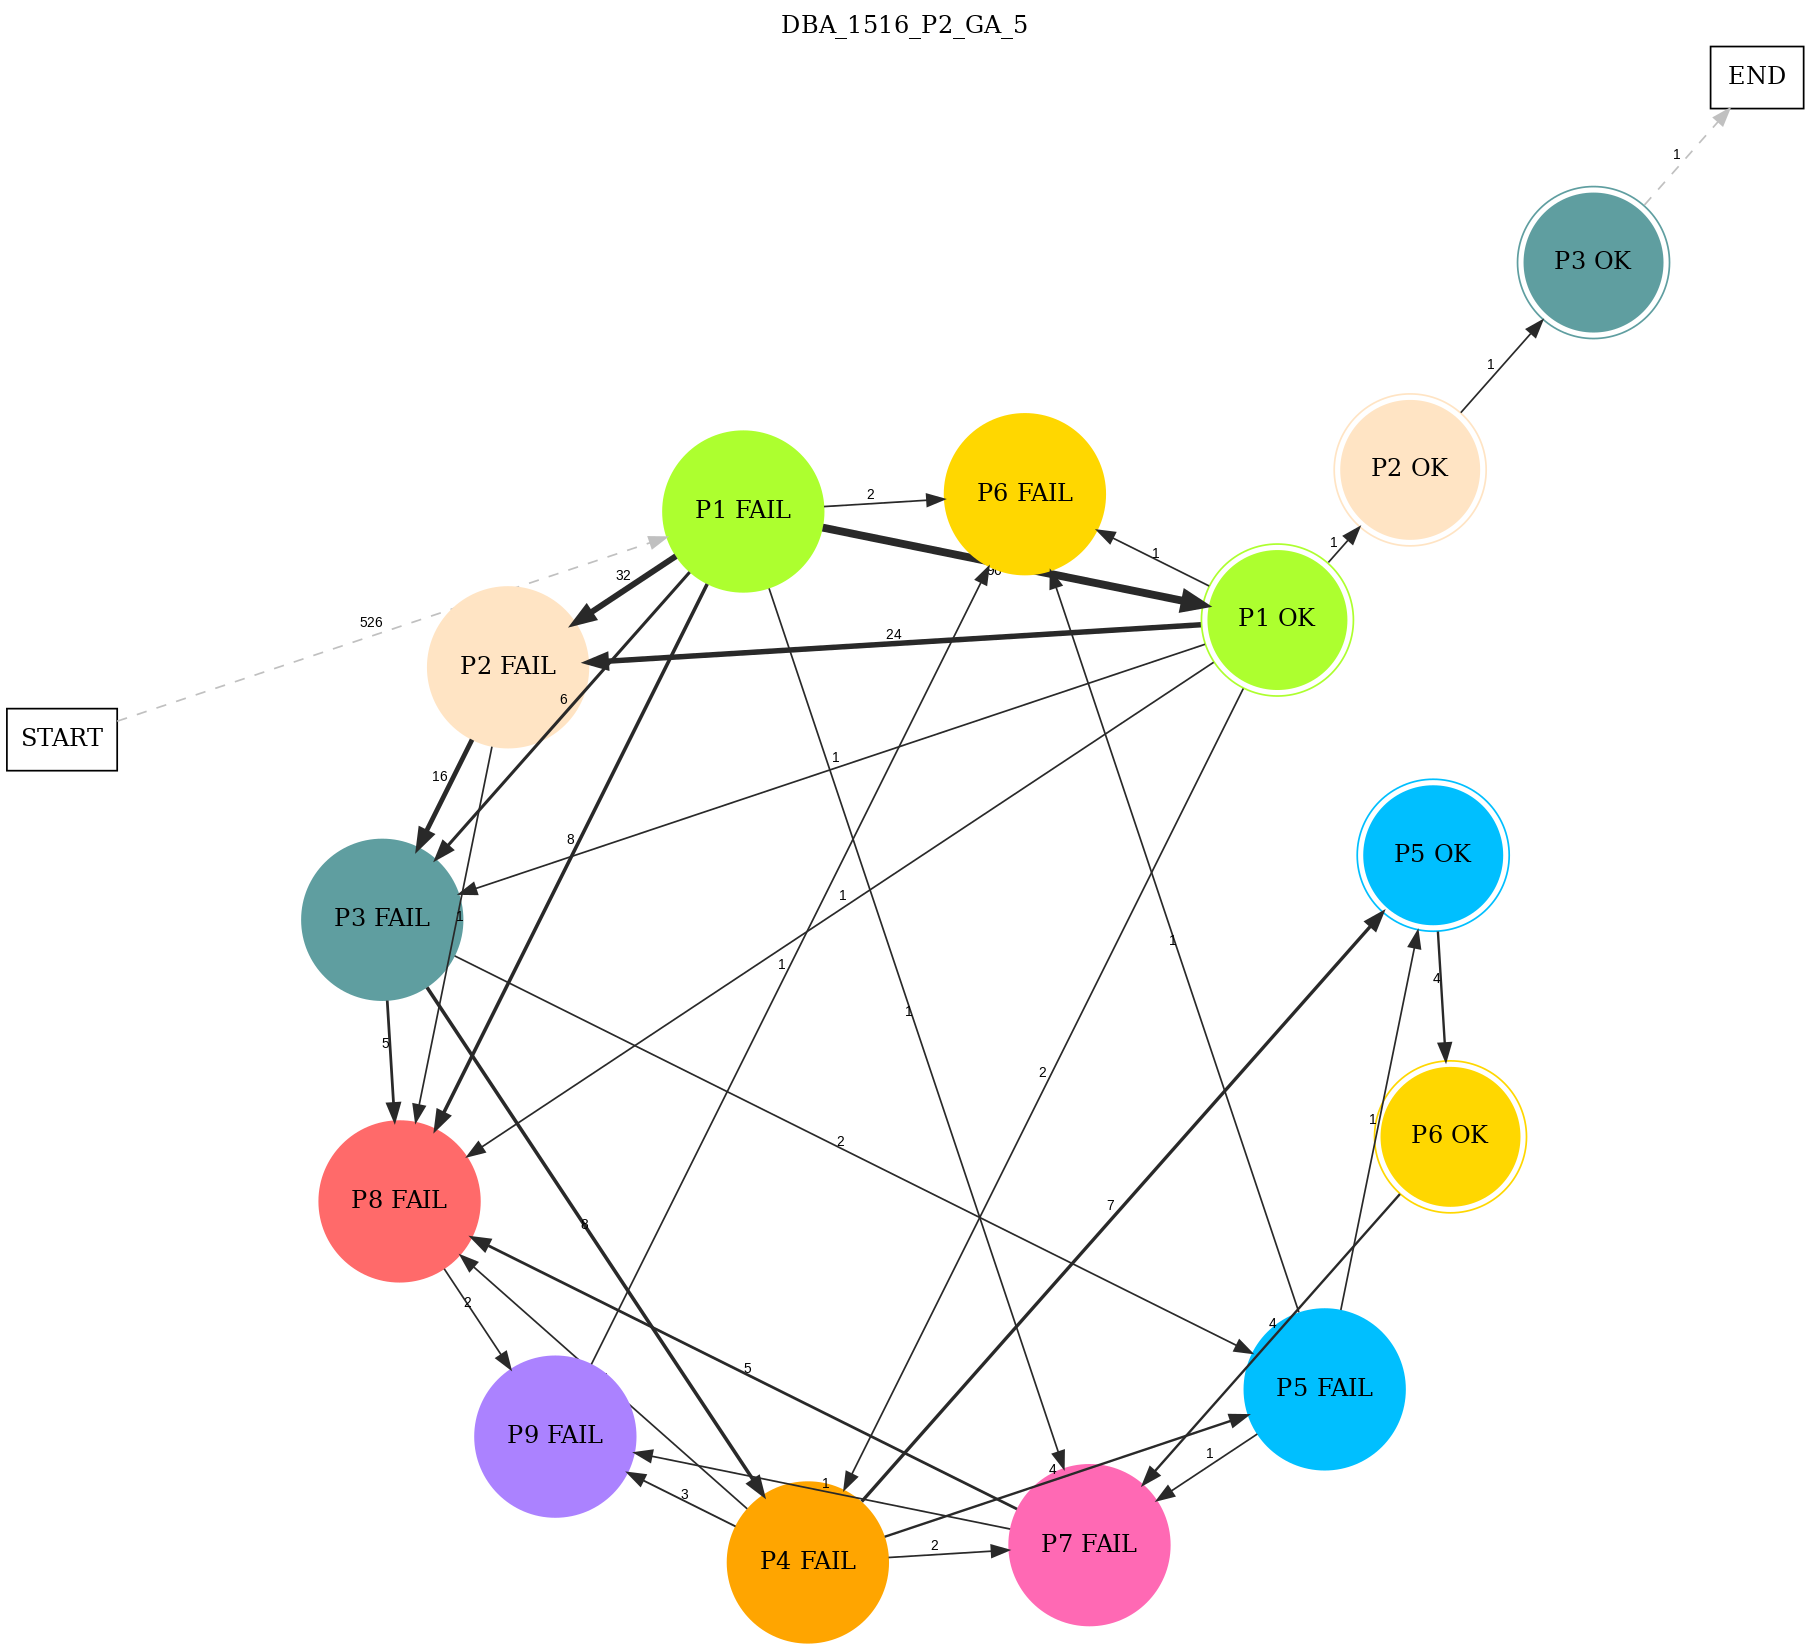
\includegraphics[width=0.7\textwidth]{implementación/DBA_1516_P2_GA_5.png} \\
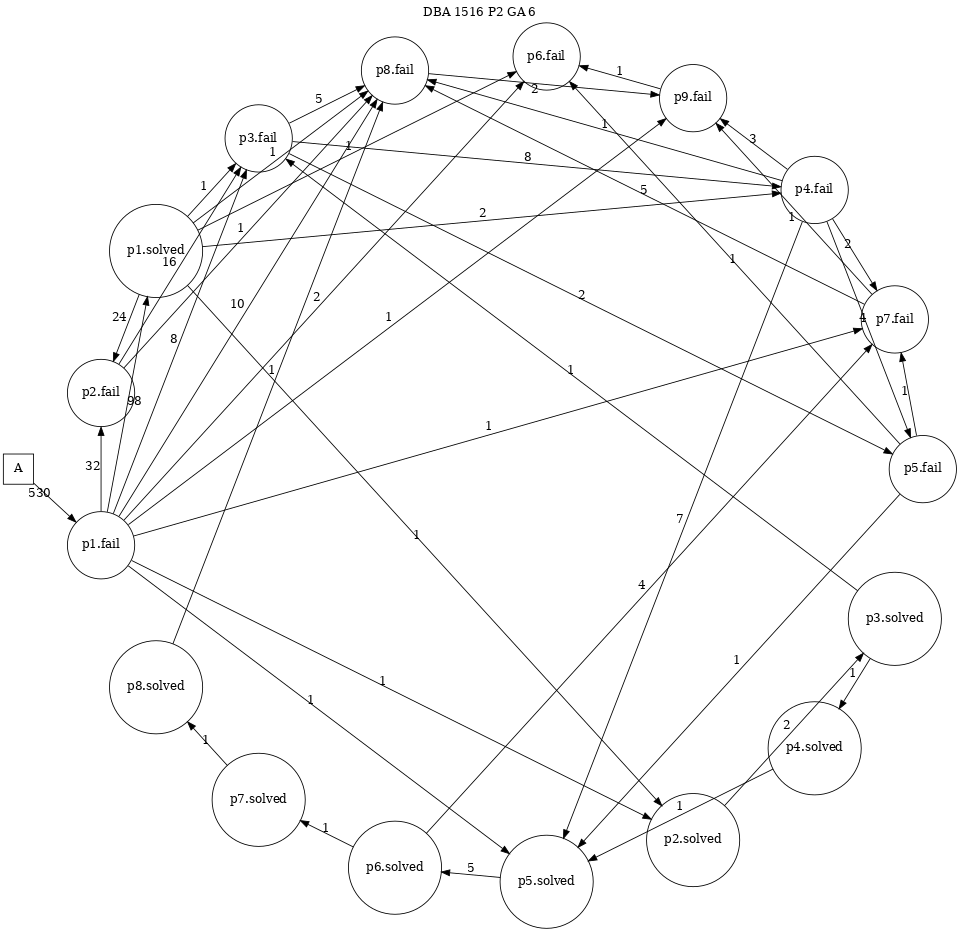
\includegraphics[width=0.7\textwidth]{implementación/DBA_1516_P2_GA_6.png}
\caption{Análisis de procesos del grupo \texttt{DBA 1516 P2 GA} (\texttt{Activity} problema-estado y \texttt{CaseId} sesión) obtenido con la implementación propia. En estos grafos los ciclos se han eliminado con el procedimiento explicado en la Sección \ref{sec:representation}.}
\label{fig:DBA1516P2GA5}
\end{figure}

\begin{figure}[H]
\centering
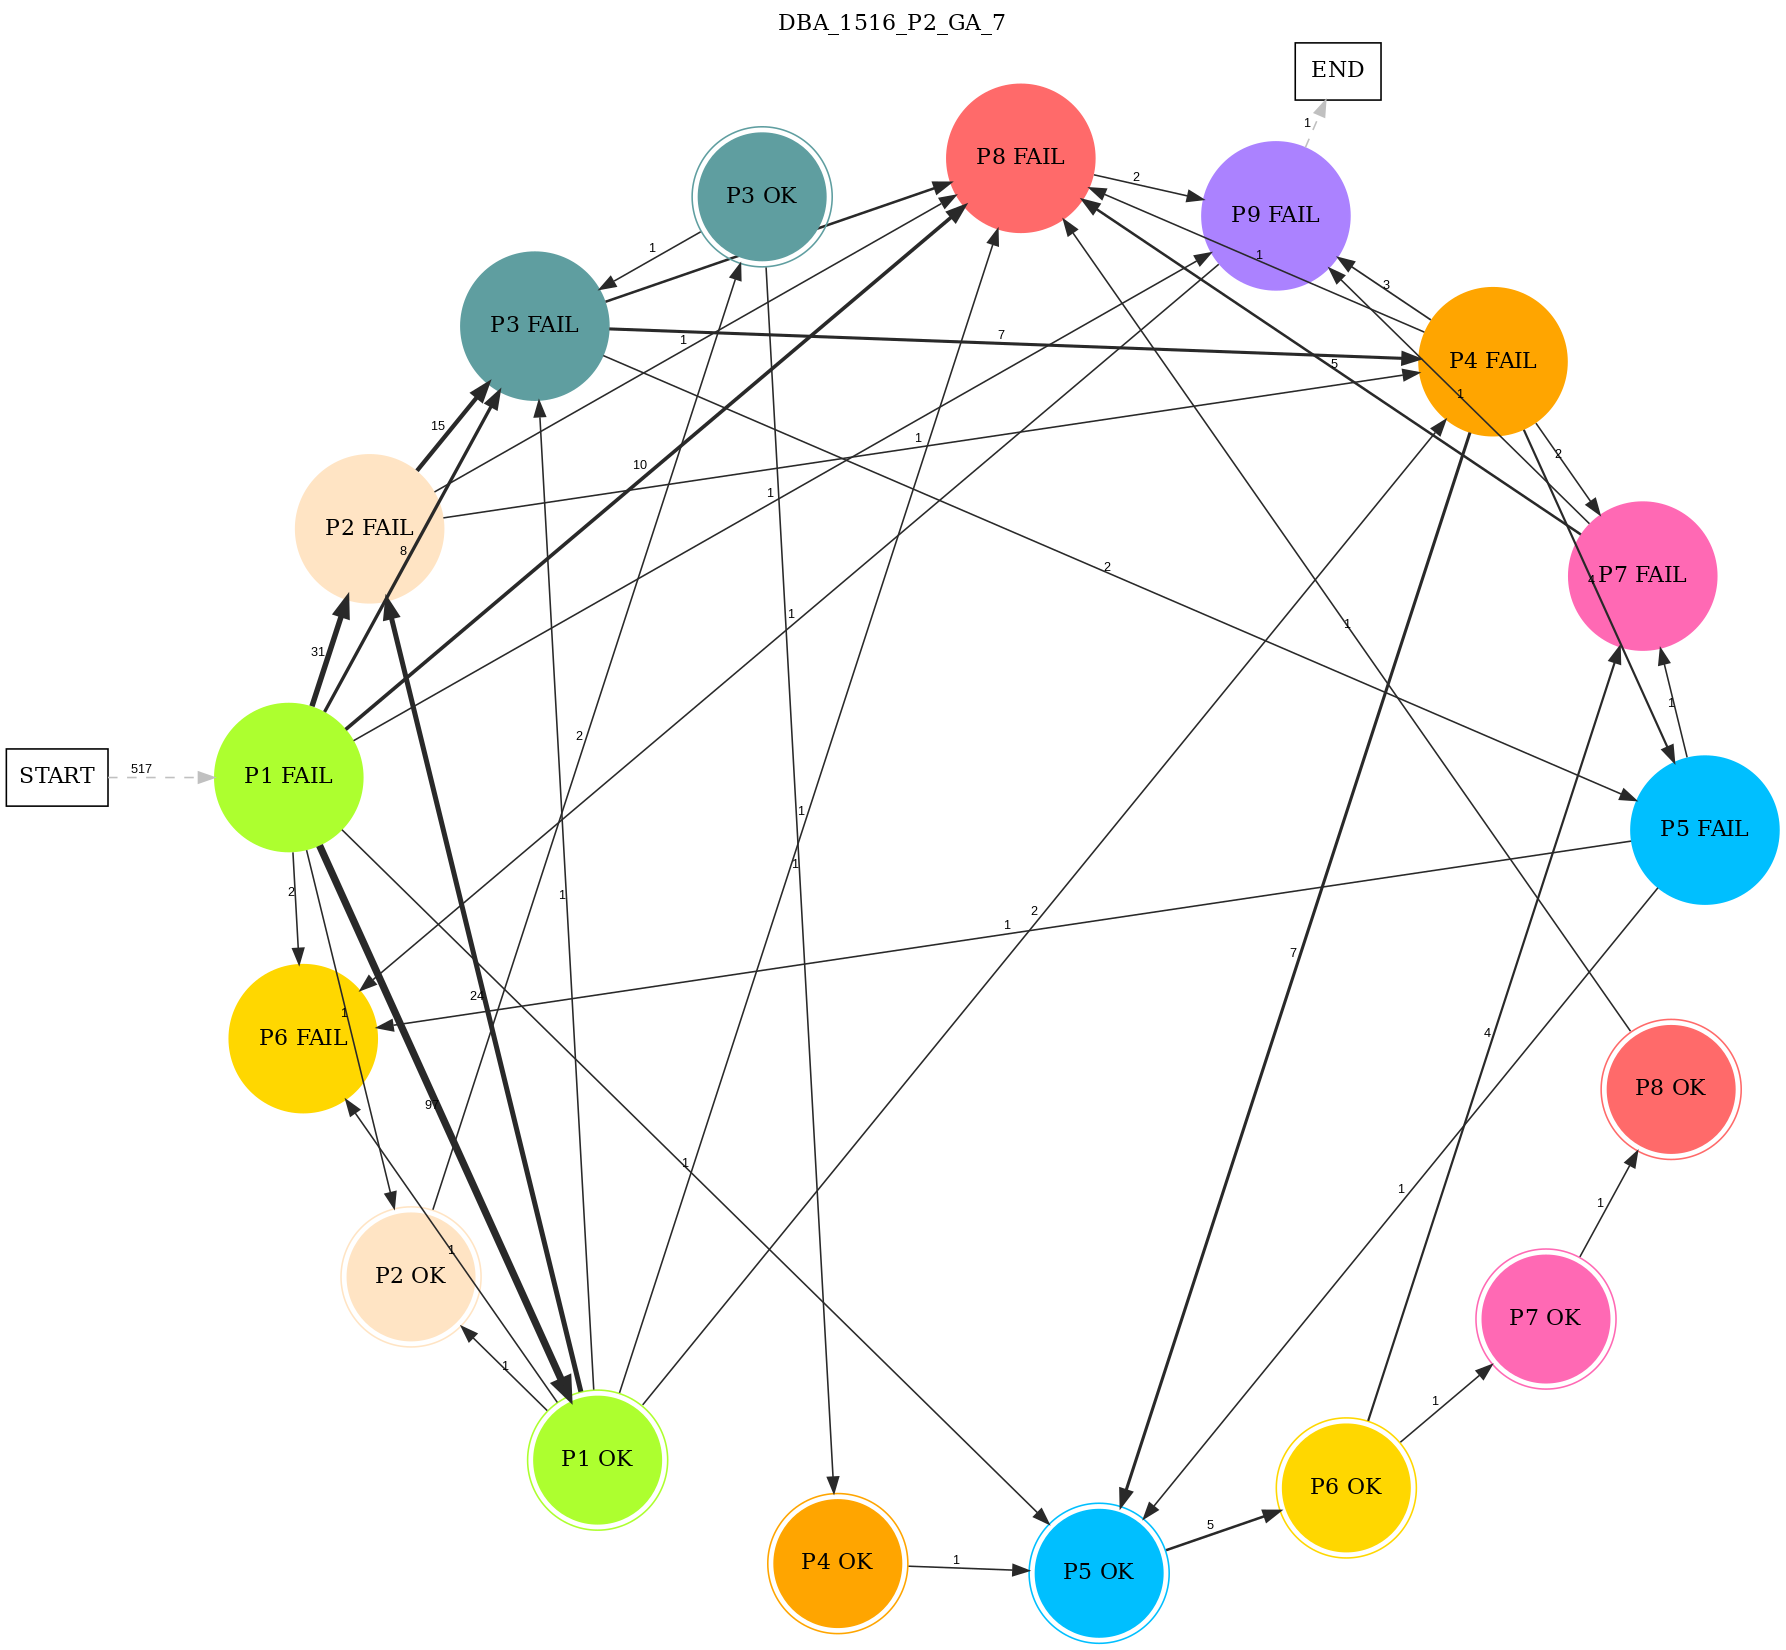
\includegraphics[width=0.7\textwidth]{implementación/DBA_1516_P2_GA_7.png} \\
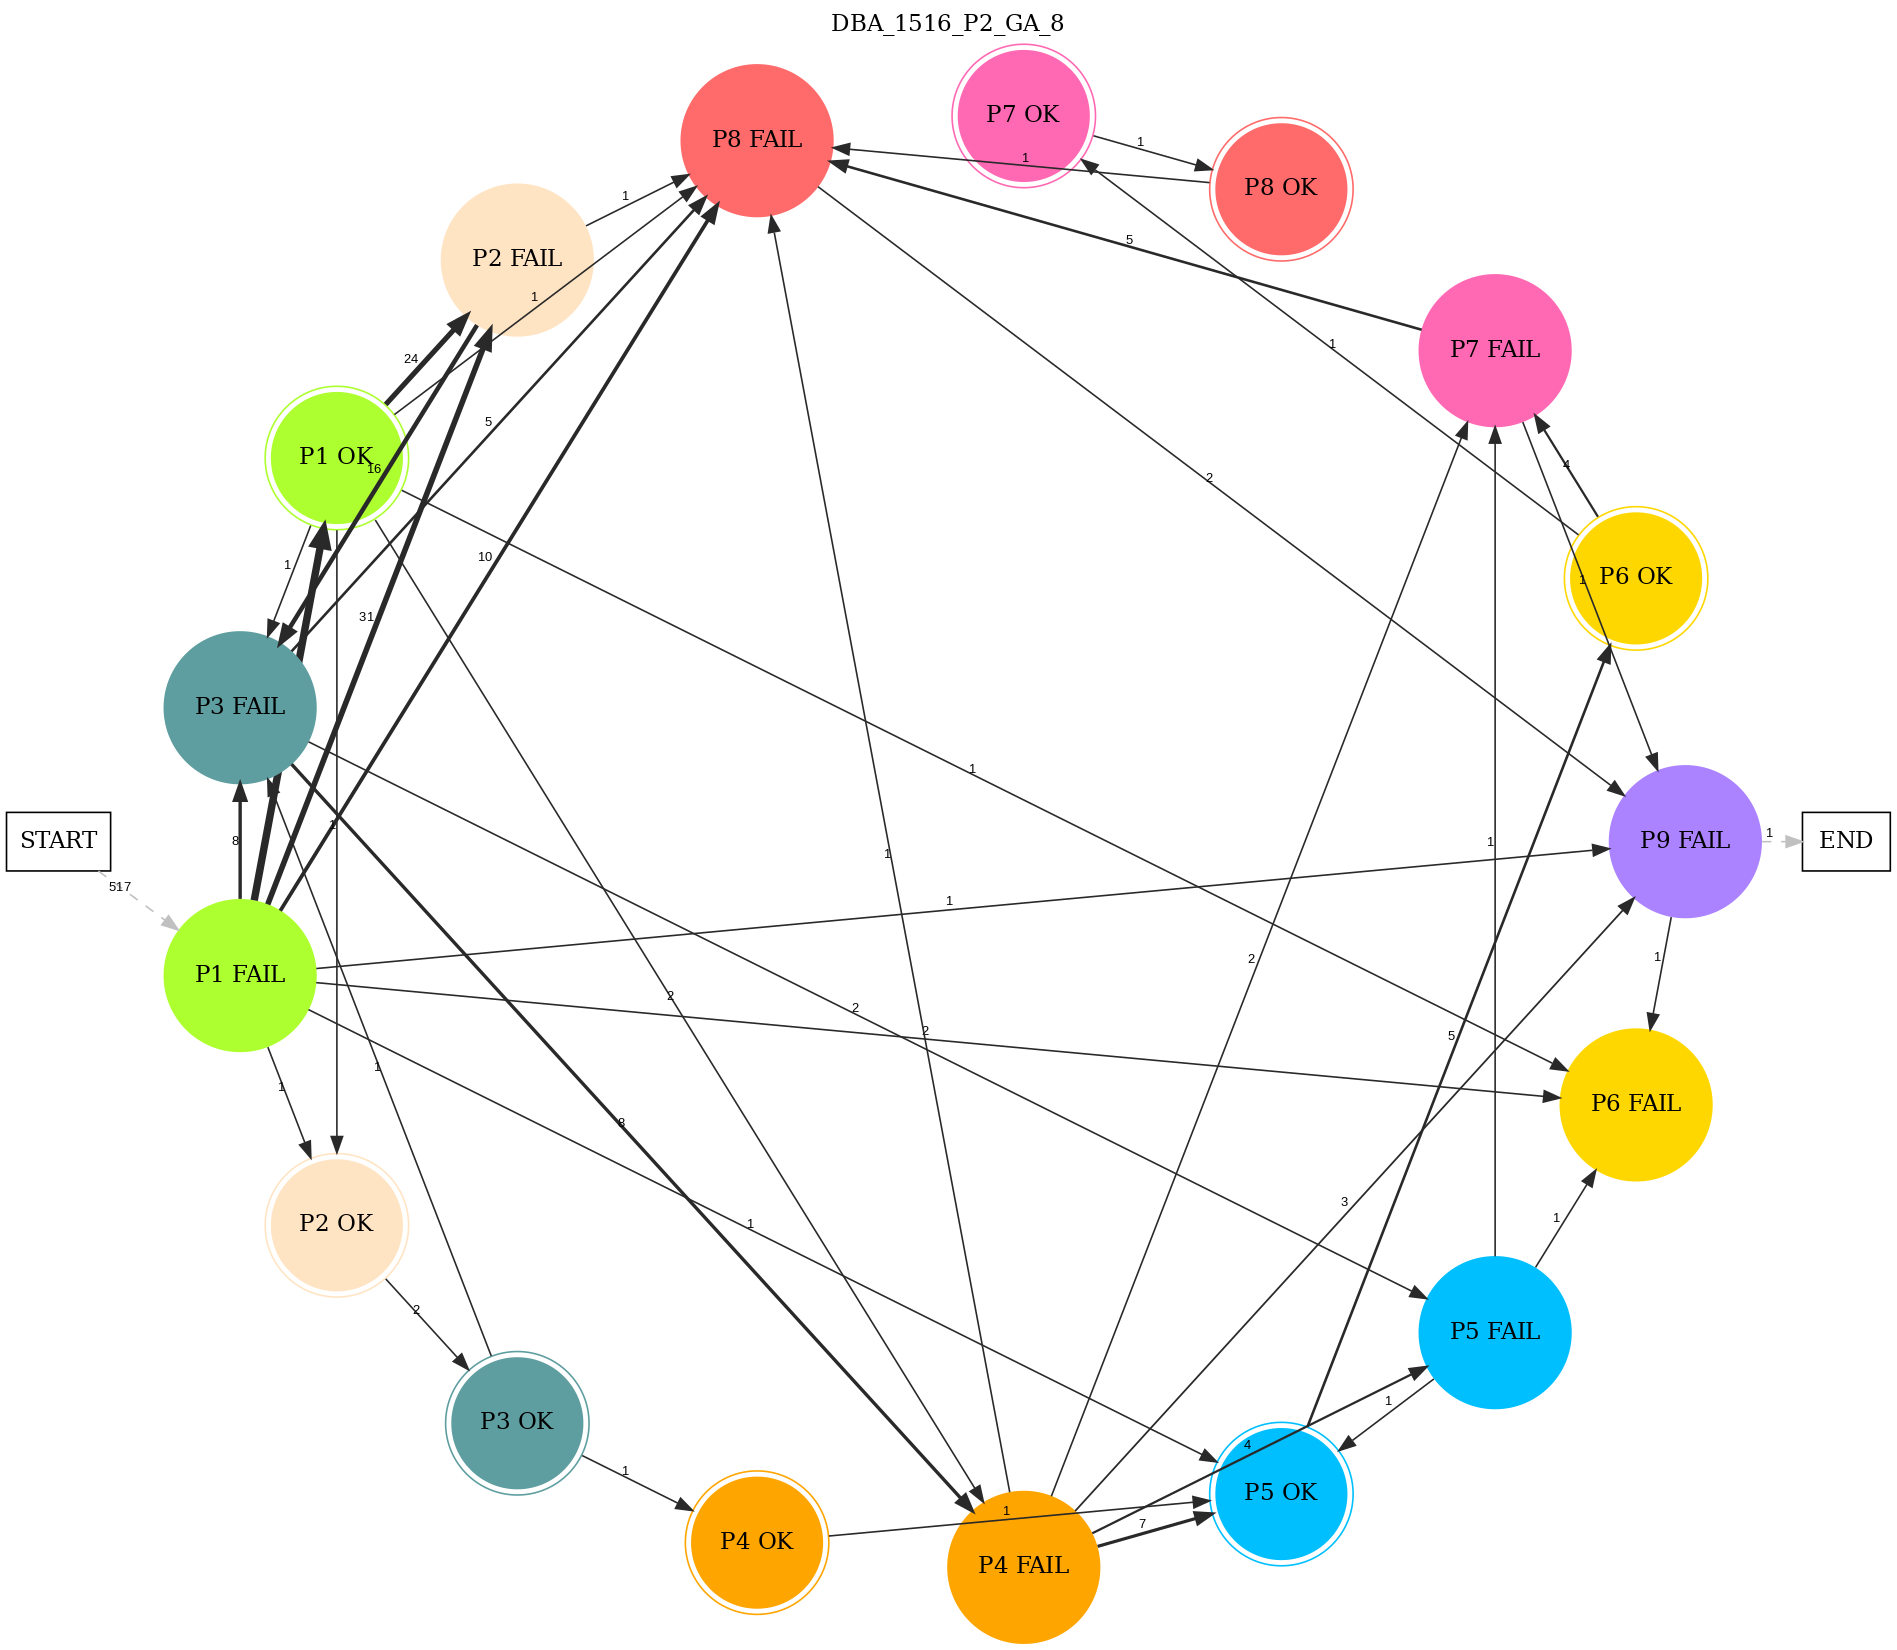
\includegraphics[width=0.7\textwidth]{implementación/DBA_1516_P2_GA_8.png}
\caption{Análisis de procesos del grupo \texttt{DBA 1516 P2 GA} (\texttt{Activity} problema-estado y \texttt{CaseId} sesión) obtenido con la implementación propia. En estos grafos los ciclos se han eliminado con el procedimiento explicado en la Sección \ref{sec:representation}.}
\label{fig:DBA1516P2GA6}
\end{figure}

\begin{figure}[H]
\centering
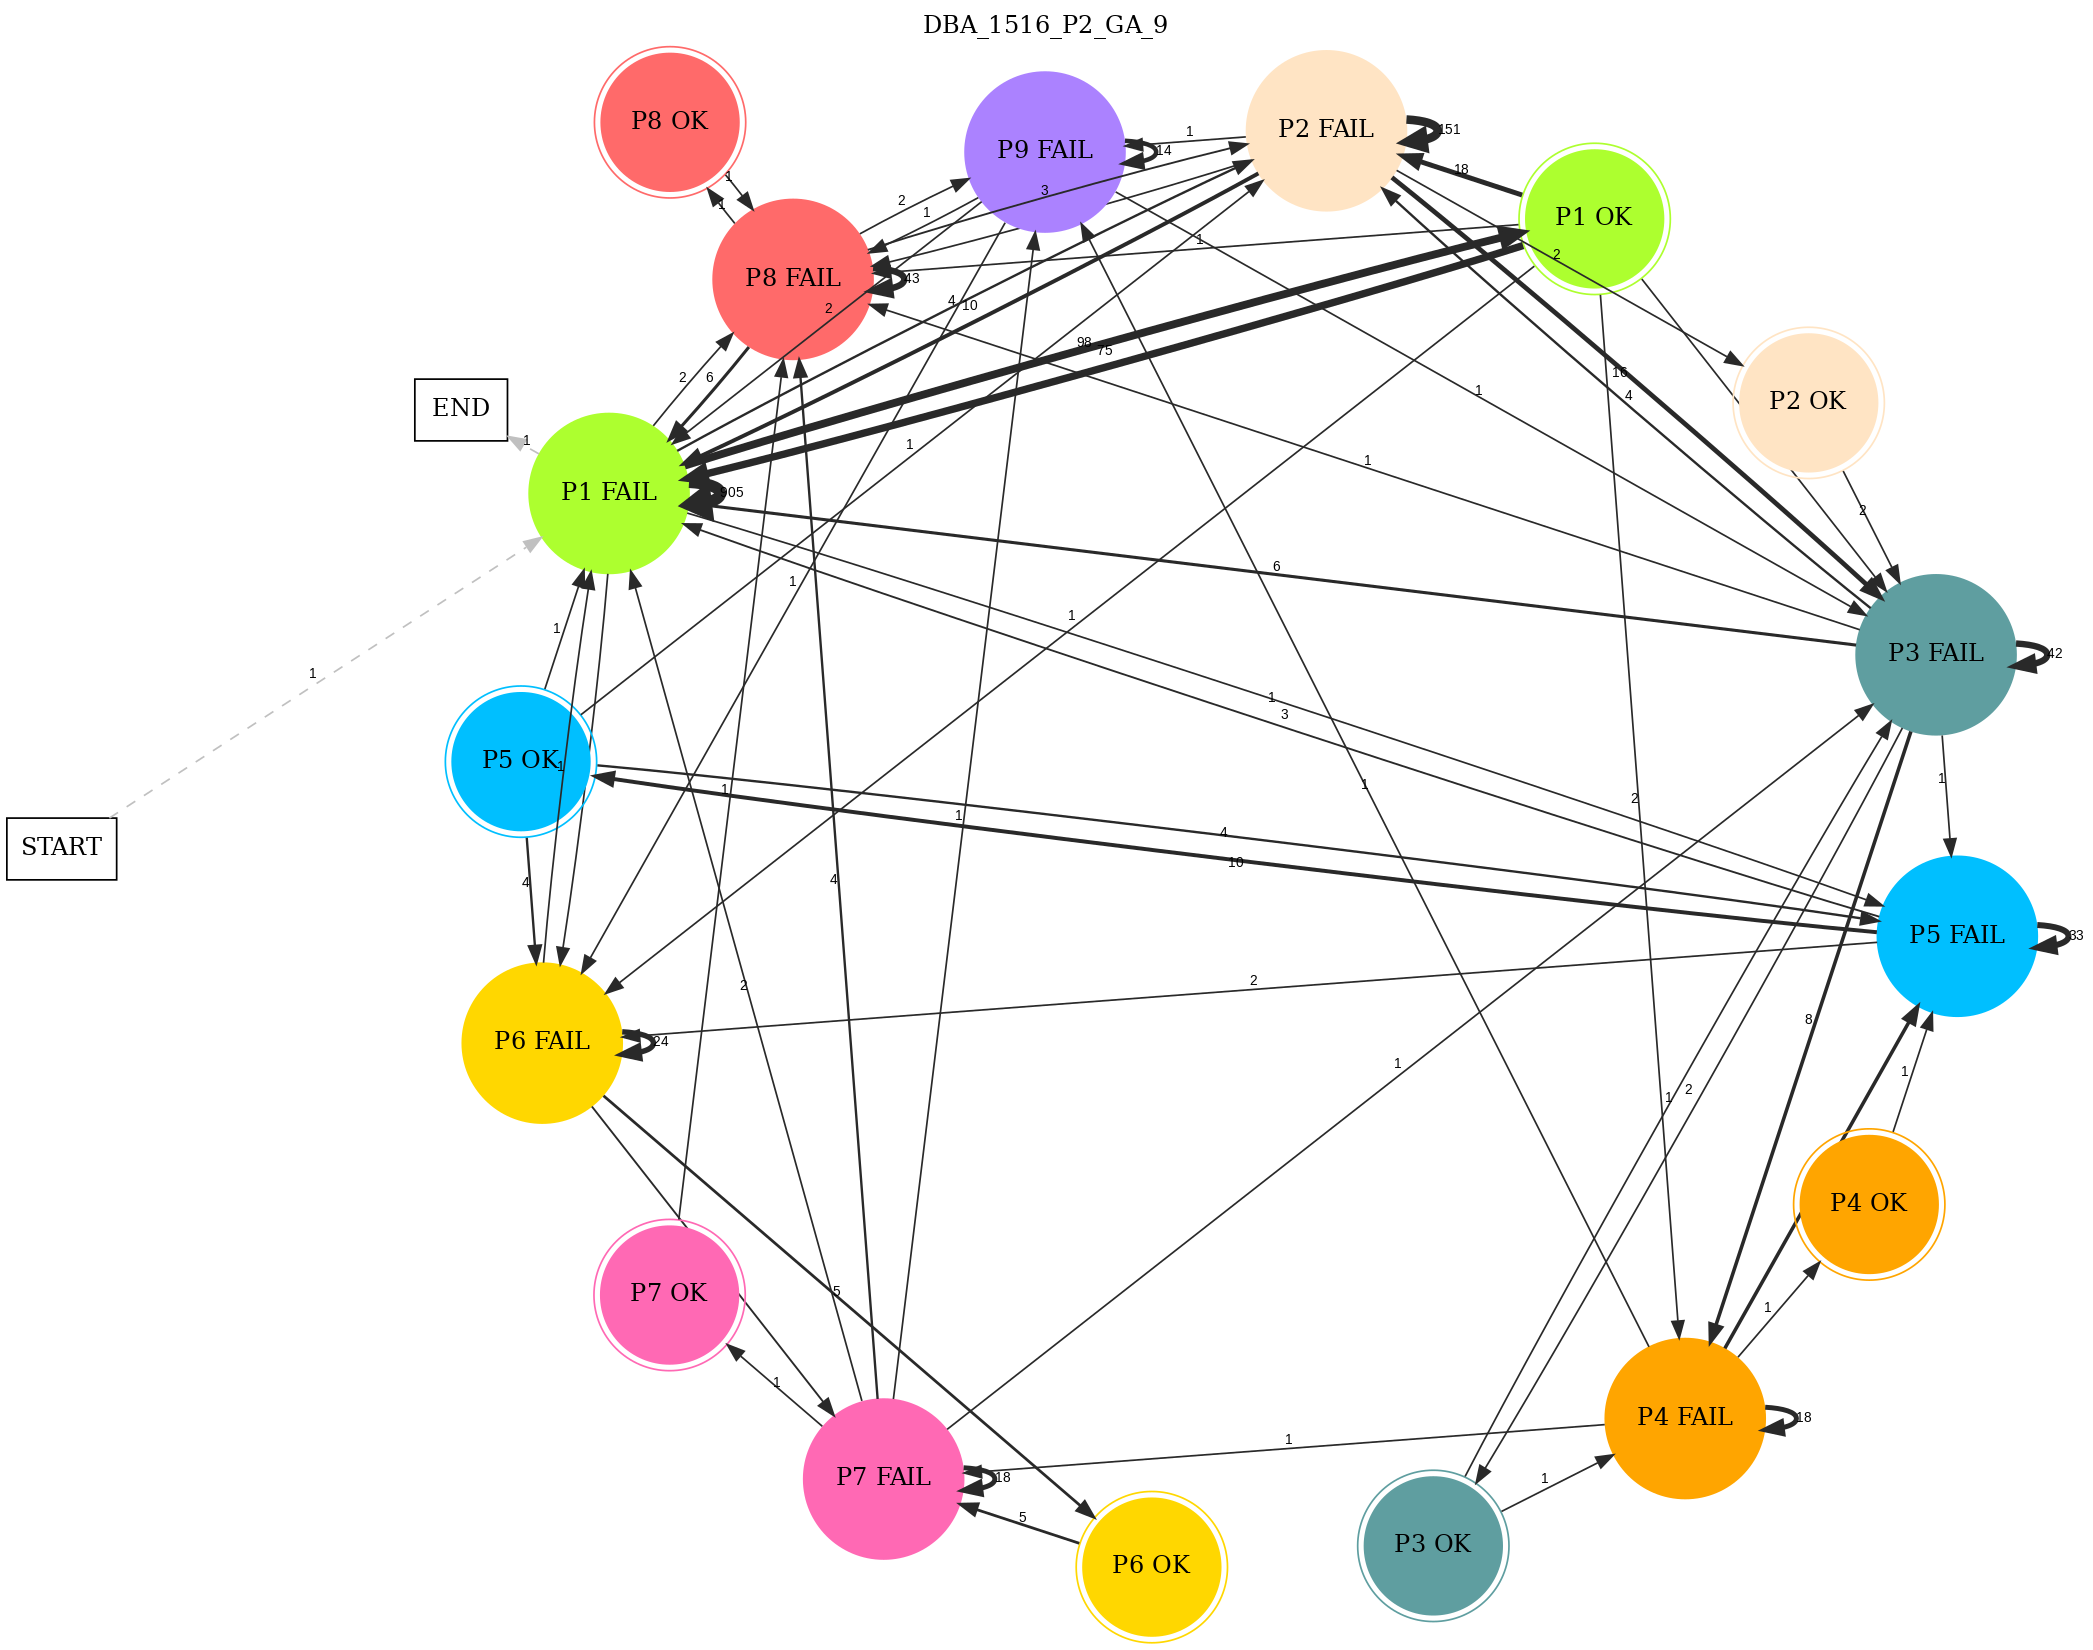
\includegraphics[width=0.7\textwidth]{implementación/DBA_1516_P2_GA_9.png} \\
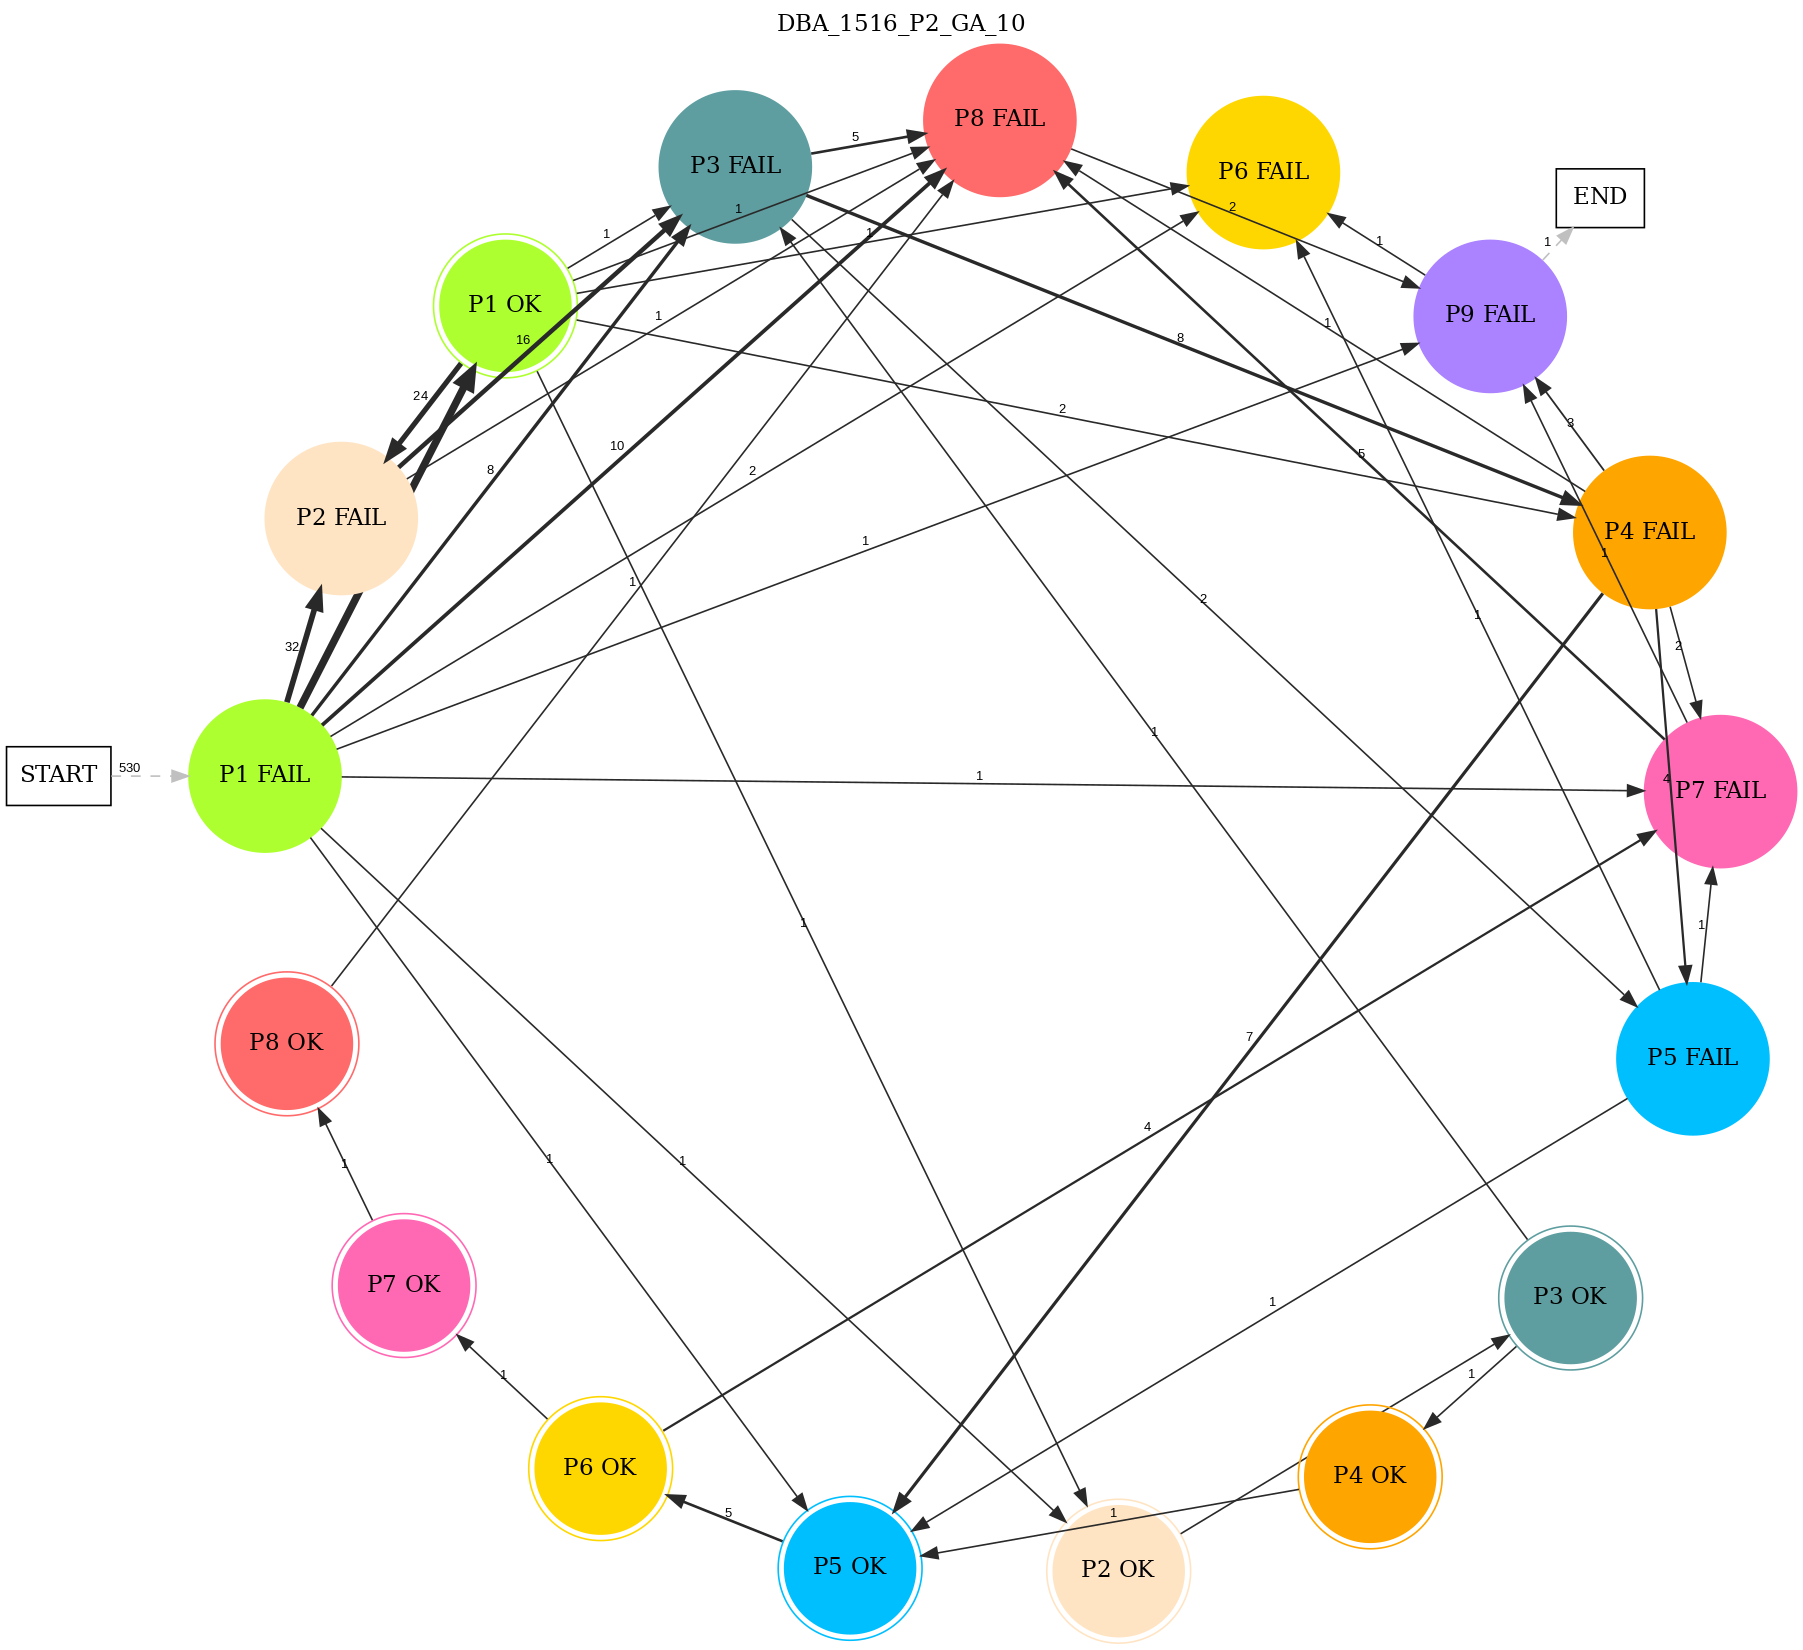
\includegraphics[width=0.7\textwidth]{implementación/DBA_1516_P2_GA_10_final.png}
\caption{Análisis de procesos del grupo \texttt{DBA 1516 P2 GA} (\texttt{Activity} problema-estado y \texttt{CaseId} sesión) obtenido con la implementación propia. En estos grafos los ciclos se han eliminado con el procedimiento explicado en la Sección \ref{sec:representation}. En este caso, el grupo \texttt{DBA 1516 P2 GA} ha resuelto únicamente $8$ de los $9$ problemas resueltos, por lo que las gráficas \texttt{DBA\_1516\_P2\_GA\_9} y \texttt{DBA\_1516\_P2\_GA\_10} son idénticas y contendrán toda la actividad registrada en el servidor de dicho grupo.}
\label{fig:DBA1516P2GA7}
\end{figure}

A partir de ahora, estos diagramos tendrán la consideración de grafos. En particular, serán grafos dirigidos y operaremos con ellos como tales. En el siguiente capítulo se expondrán los conceptos básicos de grafos y principales resultados matemáticos que se usarán en este trabajo fin de grado.